\chapter{Enzyme kinetics and ligand binding biophysical studies reveal a combined role for multiple allosteric ligands in the regulation of PKM2.}
\label{chapter:enzyme_kinetics}


\section{Introduction}
PKM2 enzyme activity is regulated by a number of intracellular metabolites. The upstream glycolytic intermediate fructose 1,6-bisphosphate (FBP) stimulates PKM2 catalysis by binding to an allosteric pocket in the C-domain of the protein \cite{Ashizawa:1990aa,Ashizawa:1991aa,Dombrauckas:2005aa,Hofmann:1975aa}. Additionally, serine (Ser) and histidine (His) increase; whereas phenylalanine (Phe), alanine (Ala), tryptophan (Trp), valine (Val) and proline (Pro) inhibit PKM2 enzyme activity by binding to a common pocket, sandwiched between the A- and the C-domains \cite{Ashizawa:1991aa,Chaneton:2012aa,Eigenbrodt:1983aa,Morgan:2013aa,Yuan:2018aa}. Crystallographic structures of PKM2 showing that the FBP- and amino acid binding pockets are \textcolor{red}{physically and chemically distinct,} suggests that PKM2 can concurrently bind to both FBP and an amino acid \cite{Chaneton:2012aa}. What remains unclear, however, is how simultaneous binding of multiple ligands with, opposing functional effects, control PKM2 enzyme activity.
%
% 
\\\\
%
%
The following chapter investigates the functional consequences of allosteric regulation by a number of regulators, both alone and in combination, on PKM2 enzyme activity. In support of \textit{in vitro} findings, we explore cellular metabolic conditions required for concurrent allosteric regulation of PKM2.
\clearpage

\section{Characterising the kinetics of FBP binding to and activation of PKM2}
Activation of PKM2 by FBP is a prototypical and long-studied example of feed-forward regulation in cellular metabolism \cite{Koler:1968aa}. Nevertheless, the mechanism of PKM2 activation is disputed; some studies have reported an increased affinity for the substrate phosphoenolpyruvate (PEP) \cite{Boxer:2010aa,Chaneton:2012aa,Jiang:2010aa,Walsh:2011aa} and others reporting changes to the rate of substrate turnover \cite{Morgan:2013aa,Yuan:2018aa}. To reconcile the differing results in the literature, and to characterise PKM2 regulation at the basal level, we started by investigating the kinetics of FBP binding and regulation of PKM2 activity.


\subsection{FBP binds to PKM2 with nanomolar affinity}
\label{subsec:fbp_binding_pkm2}
PKM2 contains three tryptophan residues, two of which (W482 and W515) are proximal to the FBP binding pocket \cite{Dombrauckas:2005aa}. Previous studies have reported that addition of FBP leads to changes to the intrinsic fluorescence emission spectrum of PK \cite{Kuczenski:1971aa}, likely resulting from side-chain conformational changes to W482 and W515 upon FBP binding \cite{Morgan:2013aa}. Therefore, FBP binding to PKM2 was measured by monitoring tryptophyl fluorescence ($\lambda_{EX} = 280$ nm,  $\lambda_{EM} = 350$ nm). 

\subsubsection{Measurements of PKM2 fluorescence suggested sub-stoichiometric FBP binding}
We found that titrating PKM2 with a stock solution of FBP resulted in a ligand concentration-dependent excitation and red-shifting of the protein emission spectrum (\textbf{Fig. \ref{fig:fbp_binding_aldolase} A}). The effect of FBP on the fluorescence of PKM2 was sufficiently large to allow for a determination of the dissociation constant from titrations of the fluorescence change. Nevertheless, an inspection of the fluorescence spectra revealed that full saturation of the PKM2 fluorescence response to FBP addition occured at ligand concentrations less than the concentration of protein used in the titration (\textbf{Fig. \ref{fig:fbp_binding_aldolase} A}), suggesting sub-stoichiometric binding despite a 1:1 stoichiometry reported in several crystal structures \cite{Dombrauckas:2005aa,Chaneton:2012aa,Anastasiou:2012aa}. We therefore hypothesised that purification of recombinant PKM2 may co-purify residual amounts of FBP produced by the \textit{E. coli} expression vector, which had been previously reported \cite{Christofk:2008aa,Gavriilidou:2018aa,Morgan:2013aa}. 

\subsubsection{Sub-stoichiometric amounts of FBP are co-purified with recombinant PKM2}
Preparations of purified recombinant PKM2 were assessed for their content of co-purified FBP using a three-step aldolase assay \cite{bergmeyer1985methods}, which couples the conversion of FBP into glyceraldehyde 3-phosphate (GA-3-P) and dihydroxyacetone phosphate (DHAP) with the oxidation of NADH by glycerol 3-phosphate dehydrogenase (G-3-PDH), requiring the conversion of GA-3-P to DHAP by triosephosphate isomerase (TPI) as an intermediate step (\textbf{Fig. \ref{fig:fbp_binding_aldolase} B}). The assay was calibrated by quantifying molar amounts of FBP from a known solution of the compound made up from powder (\textbf{Fig. \ref{fig:fbp_binding_aldolase} C}). Subsequent quantitation of FBP in several independent preparations of purified PKM2, following heat-precipitation of the protein, revealed that up to 77.5 \% of purified PKM2 was pre-bound to FBP (\textbf{Fig. \ref{fig:fbp_binding_aldolase} D} and \textbf{E}), consistent with previous reports of FBP co-purification with PKM2 \cite{Gavriilidou:2018aa,Christofk:2008aa}. Many attempts to purify recombinant PKM2 under denaturing conditions, and thereby remove co-purified ligand, were unsuccessful (data not shown). Therefore, all subsequent experiments were performed with preparations of PKM2 with less than 25 \% of the protein pre-bound to FBP, so that experimental data could be interpreted consistently. Experiments performed on purified PKM2 in the absence of any added ligands, though containing quantified sub-stoichiometric amounts of FBP, are denoted with an asterisk (Apo$\ast$).

\subsubsection{Determination of the free protein concentration was used to calculate the $K_{D}^{FBP}$}
Quantification of the FBP-PKM2 saturation status using the aldolase assay allowed for an estimate of the concentration of free protein in the purified PKM2 sample, which was essential for accurately calculating the binding constant in the ligand titration experiment because the fluorescence signal is produced by the \textit{free} protein $P_{0}$ upon association with the \textit{free} ligand $L_{0}$ in solution. A variable proportion of the total PKM2 ($P_{total}$) was sequestered in a protein-ligand complex $PL$ and would therefore not produce a fluorescence change upon further addition of the ligand. Therefore, the free protein concentration of a given preparation of PKM2 could be calculated:
%
%
\begin{equation}
P_{0} = P_{total} -  PL
\end{equation}
%
%
It was unclear, however, whether sub-stoichiometric pre-occupancy of FBP meant that ligand binding was distributed amongst the protomers, producing a mixed population of tetramers with varying FBP-binding stoichiometries (0:4, 1:4, 2:4, 3:4 and 4:4), or whether a fixed percentage of PKM2 tetramers were fully bound to FBP. The distribution of stoichiometries in the starting material was likely determined by the cooperativity of FBP binding to PKM2; in an infinitely cooperative system, binding of a limiting pool of ligand to a multi-site oligomeric protein would be expected to be all or none. Nevertheless, it was assumed that the binding affinities of FBP to each of the four structurally identical pockets in the PKM2 homo-tetramer was identical, and produced equivalent fluorescence spectral changes upon ligand binding. Moreover, it was posited that the PKM2 fluorescence change was a result of ligand binding only, and that any potential oligomeric changes would not contribute to the emission spectrum. Therefore, the changed PKM2 fluorescence signal, observed upon addition of FBP, is given by a mixture of fluorescence signals from $P_0$ and $PL$:
%
%
\begin{equation}
S_{obs} = S_P \cdot [P_0] + (S_{PL} - S_{P}) \cdot [PL]
\label{equ:fluorescence_signal}
\end{equation} 
%
%
where $S_{P}$ and $S_{PL}$ are optical properties of $P_0$ and $PL$, respectively. The concentration of $PL$ at equilibrium is given by:
%
%
\begin{equation}
[PL] = \frac{(K_{D} + [P_{0}] + [L_{0}]) - \sqrt{(K_{D} + [P_{0}] + [L_{0}])^{2} - 4([P_{0}] [L_{0}])}}{2}
\end{equation}
%
%
where $K_D$ is the dissociation constant of the FBP-PKM2 interaction. Substituting the expression for $[PL]$ back into Equ. \ref{equ:fluorescence_signal}:
\begin{equation}
S_{obs} = S_{P}[P_{0}] + (S_{PL} - S_{P}) \cdot \frac{(K_{D} + [P_{0}] + [L_{0}]) - \sqrt{(K_{D} + [P_{0}] + [L_{0}])^{2} - 4([P_{0}][L_{0}])}}{2}
\label{equ:mass_action}
\end{equation}
%
%
After correcting for the partial pre-occupancy of FBP, a solution for the quadratic function $S_{obs}(S_{P}, S_{L}, S_{PL}, P_{0}, L_{0}, K_{D})$ (Equ. \ref{equ:mass_action}) was calculated using a non-linear least squares procedure to provide an estimate of the dissociation constant $K_{D}$. The calculation of the binding affinity of a protein-ligand interaction was automated in an R package \textit{ligBind} (see Methods section \ref{subsec:methods_fbp_binding} for details and software tutorial). An average apparent $K_D^{FBP}$ of (21.4 $\pm$ 9.0) nM was estimated from a total of six replicate FBP binding measurements (\textbf{Fig. \ref{fig:fbp_binding_aldolase} F}).
%
%
%
%%% FIGURE
%
\begin{figure}[!ht]
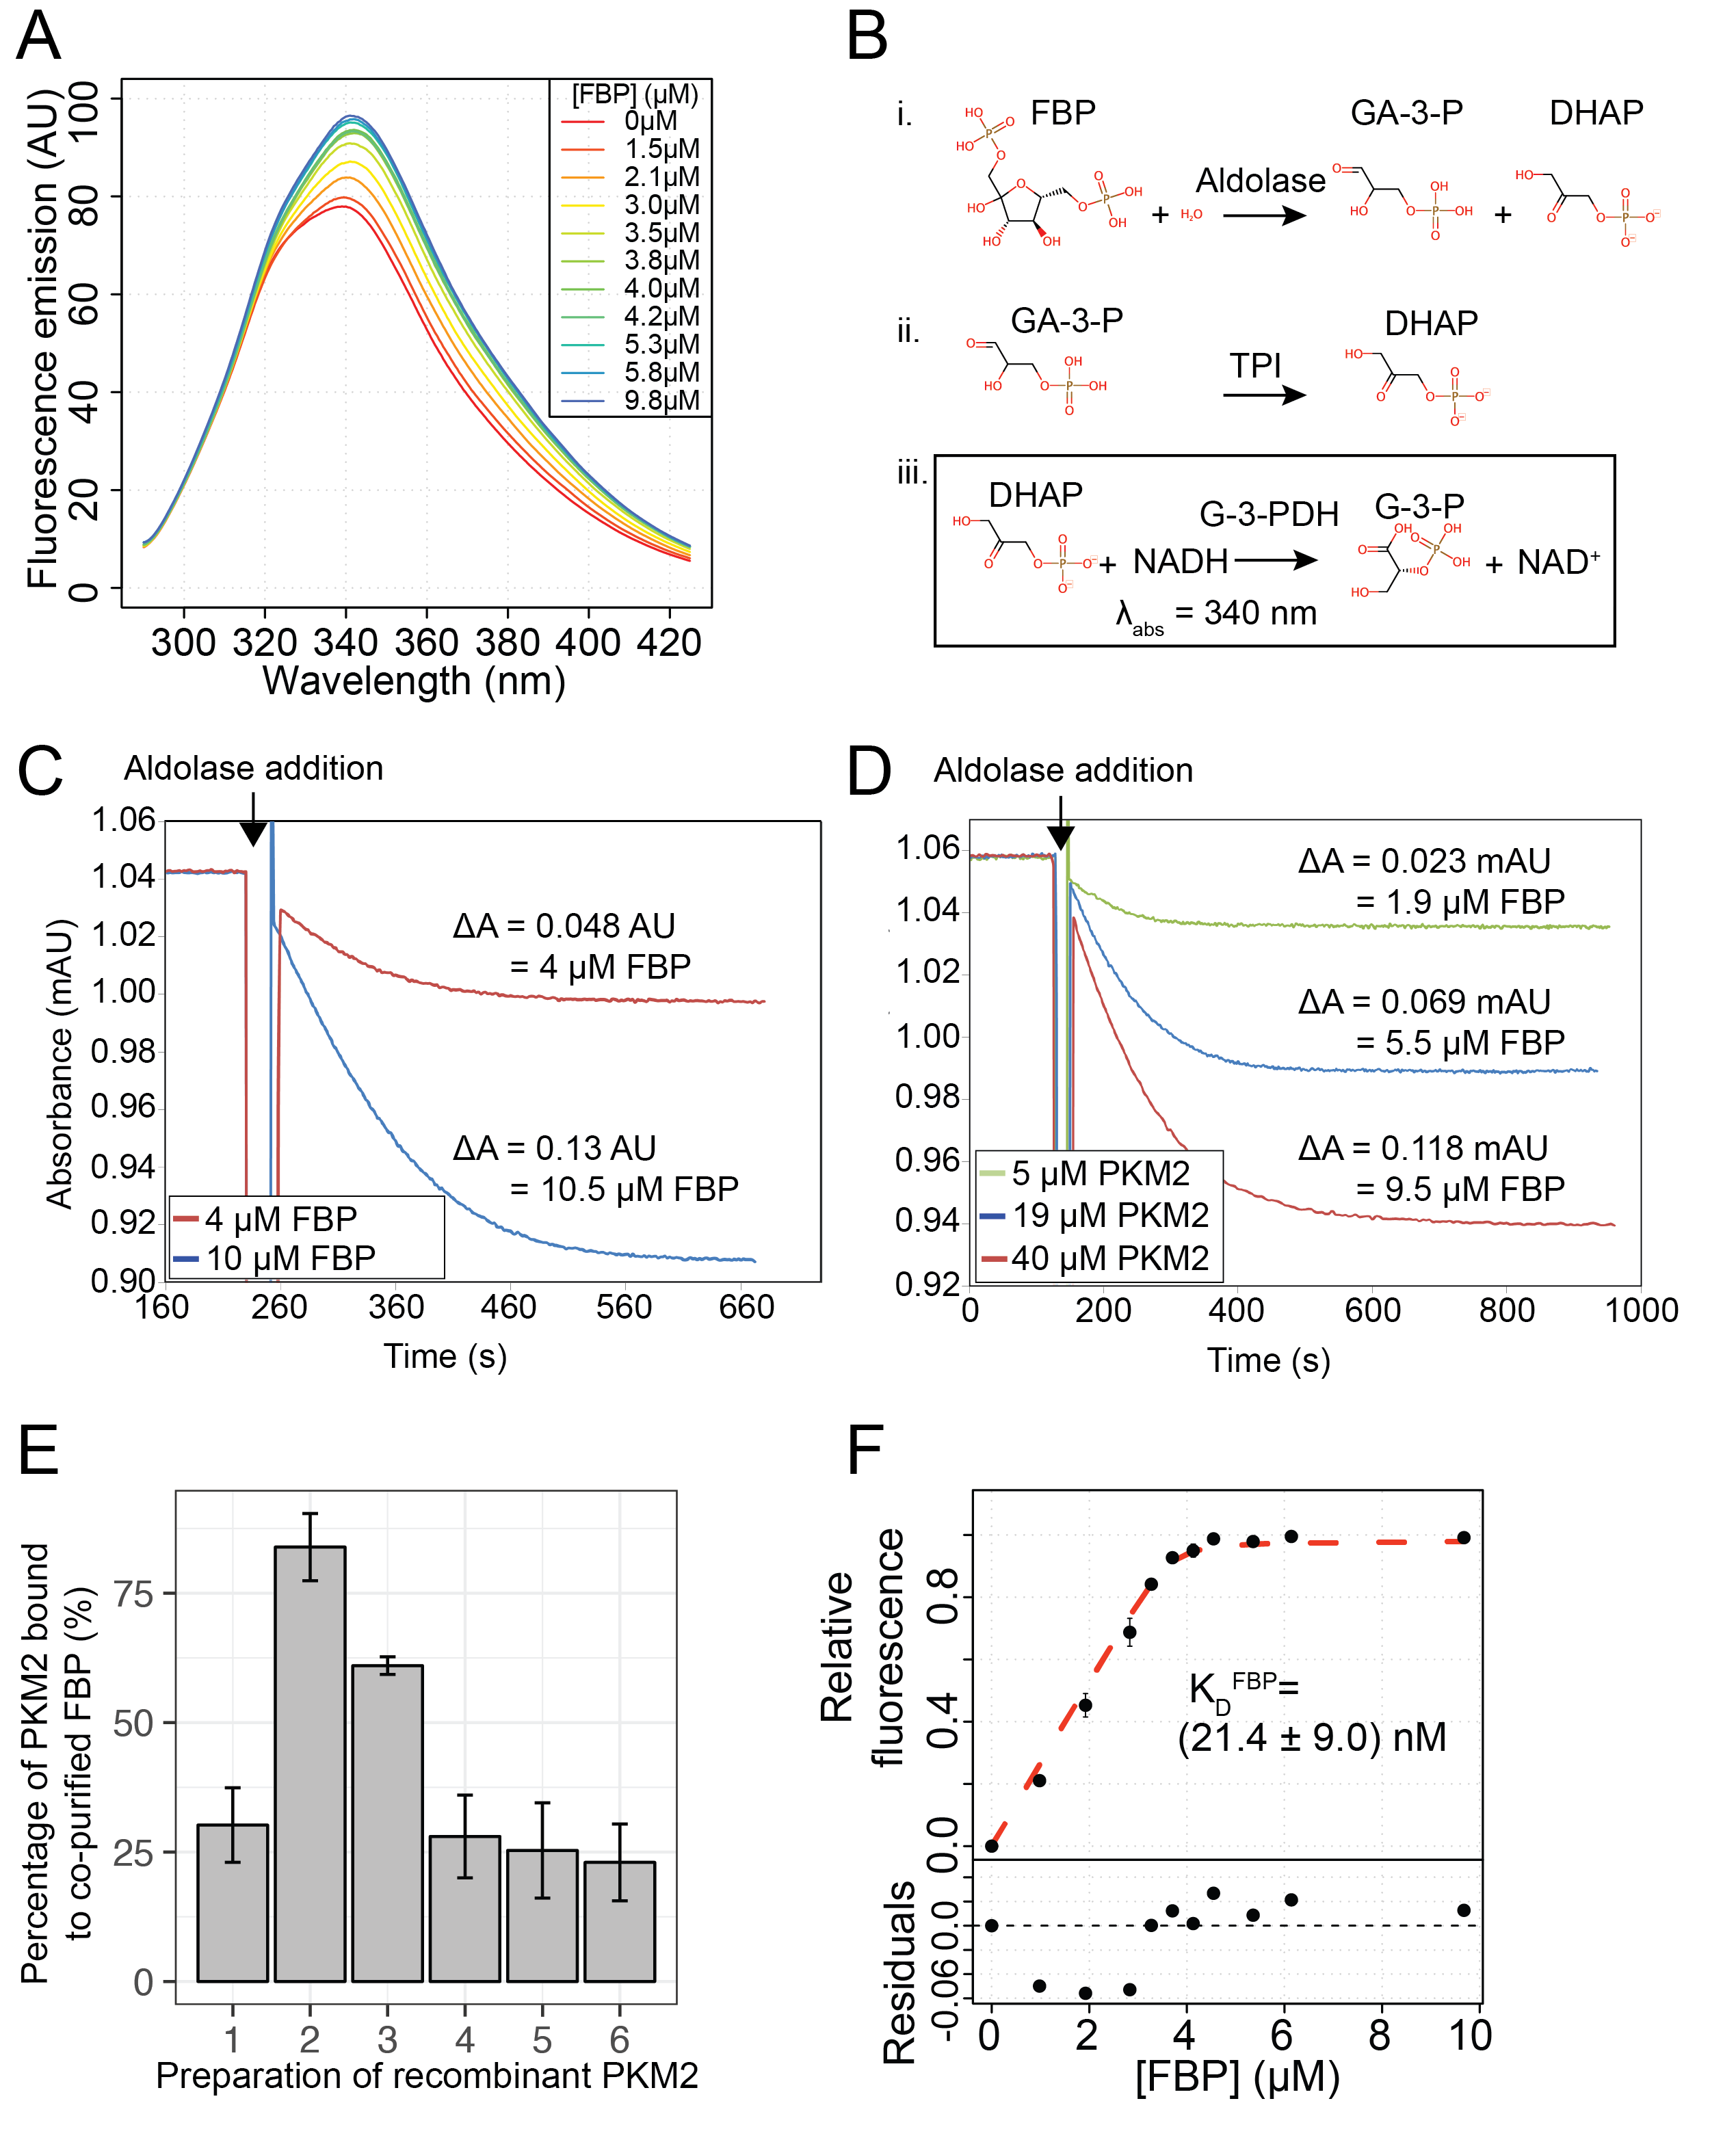
\includegraphics[scale=0.55]{ch4_fig1_fbp_binding.png}
\caption[FBP binds to PKM2 with nano-molar affinity.]{\textbf{FBP binds to PKM2 with nano-molar affinity.} \textbf{(A)} Fluorescence spectra of human PKM2 in 10 mM HEPES pH 7.5, 100 mM KCl, 10 mM MgCl$_2$ at 20 \textdegree C. A protein concentration of 5 $\mu$M was used for all curves and the concentration of FBP is specified in the legend. \textbf{(B)} Molar amounts of FBP co-purified with recombinant PKM2 were quantified using a three-step enzymatic assay, as described in the text. \textbf{(C)} Calibration of the aldolase assay to estimate the sensitivity for measuring amounts of co-purified FBP. The assay was tested by adding 4 $\mu$M or 10 $\mu$M purified FBP. \textbf{(D)} Preparations of 5 $\mu$M (green), 19 $\mu$M (blue) and 40 $\mu$M (red) of purified PKM2 were heat-precipitated at 90 \textdegree C to release any co-purified FBP. The supernatant was subsequently analysed for its molar contents of FBP, as previously described in (B). \textbf{(E)} Quantitation of the percentage saturation of PKM2 with FBP in six independent preparations of purified recombinant PKM2. \textbf{(F)} Binding was monitored from spectroscopic measurements of PKM2 fluorescence emission with increasing concentrations of FBP. The relative changes to emission at 325 nm and 350 nm is plotted against the concentration of added FBP. The binding affinity was calculated, as described in the text. Means and standard deviations from six separate experiments are plotted.}
\label{fig:fbp_binding_aldolase}
\end{figure}
%
%
\clearpage

\subsection{Technical note: the protein concentration determines the error associated with the $K_D$ of PKM2-FBP binding}
Experimental measurements of PKM2 fluorescence in Section \ref{subsec:fbp_binding_pkm2} were necessarily performed at a protein concentration of 5 $\mu$M because of the limited quantum-yield of tryptophan. As such, $P_0$ was approximately 220-times greater than the estimated $K_D^{FBP}$. Measurements of ligand binding are known to be increasingly imprecise under conditions where $[P_{0}] >> K_{D}$ because small additions of $L$ are sequestered into the $PL$ complex (i.e $L_{0} << L_{total} \simeq PL$) \cite{Hulme:2010aa,Pollard:2010aa}, which was accounted for in our numerical treatment of the binding data (see Section \ref{subsec:fbp_binding_pkm2}). We therefore questioned to what extent using a protein concentration orders of magnitude in excess of the binding constant would contribute the imprecision of the affinity estimate.
%
\\\\
%
To this end, a numerical approach was employed whereby theoretical ligand-protein binding data were simulated using the ligBind::simtitr() function within a new R package \textit{ligBind} (see Methods section \ref{subsec:methods_fbp_binding}). Binding data were simulated over a range of increasing $P_{0}$ and a defined \textit{theoretical} $K_D$ of 1 $\mu$M. The simulated binding data were subsequently fit using Equ. \ref{equ:mass_action} to estimate a \textit{calculated} $K_D$, which was compared to the initialised \textit{theoretical} $K_D$ to determine the percent error of the affinity calculate for a given $P_0$. Where the theoretical $K_{D} >> P_{0}$, the transition between unbound and fully bound is achieved over a gradient of ligand concentrations (\textbf{Fig. \ref{fig:binding_simulation} A}). In contrast, where $K_{D} << P_{0}$, the resulting quadratic function $S_{obs}(S_{P}, S_{L}, S_{PL}, PL, K_{D})$ has a sharp apex, leading to a higher percent error (\textbf{Fig. \ref{fig:binding_simulation} B}).
%
%
\\\\
%
%
Next, the $K_D$ was calculated for simulated binding data over a range of $[P_{0}]$ up to 250 $\mu$M. We found that, where $[P_0] \le 50 \cdot K_{D}$ the calculated binding affinity was approximately equivalent to the true binding affinity when fitted with the quadratic function $S_{obs}(S_{P}, S_{L}, S_{PL}, PL, K_{D})$ (\textbf{Fig. \ref{fig:binding_simulation} C}), resulting in a negligible percent error of the apparent affinity. As the free protein concentration was increased such that $P_0 \ge 50 \cdot K_{D}$, we observed a non-linear increase in the calculated binding affinity ($\mu K_D$) (\textbf{Fig. \ref{fig:binding_simulation} C}). 
%
%
\\\\
%
%
For comparison, the same binding data were fitted with a hyperbolic function of the form:
%
%
\begin{equation}
S_{obs} = \frac{[L_{total}]}{[L_{total}] + K_{D}}
\label{equ:hill_equation}
\end{equation}
%
%
similar to other classical fitting methods, where binding is expressed as a function of the total ligand concentration ($[L_{total}]$), but does not account for the concentration of the three species present at equilibrium ($P_0$, $L_0$ and $PL$). Fitting simulated binding data over a range of $P_0$ using a classic graphical approach in Equ. \ref{equ:hill_equation}, high $P_0$ leads to an unacceptable percentage error of $>$ 10000 \% (\textbf{Fig. \ref{fig:binding_simulation} D}), which dwarfs the relatively moderate error we obtain by fitting with the quadratic function in Equ. \ref{equ:mass_action} (\textbf{Fig. \ref{fig:binding_simulation} C}). 
%
%
\\\\
%
%
Therefore, given the experimental limitations (outlined above) that precluded us from using PKM2 concentrations close to the $K_D$, the fit of the quadratic equation permitted the use of our binding data to determine $K_D$s. Importantly, \textbf{Fig. \ref{fig:binding_simulation} C} suggests that at higher $P_0$, the calculated $K_{D}^{FBP}$ reported in Section \ref{subsec:fbp_binding_pkm2} is likely higher than the theoretical $K_D$ (i.e. FBP binds even tighter than our data suggest). 
%
%
%%% FIGURE
%
\begin{figure}[!ht]
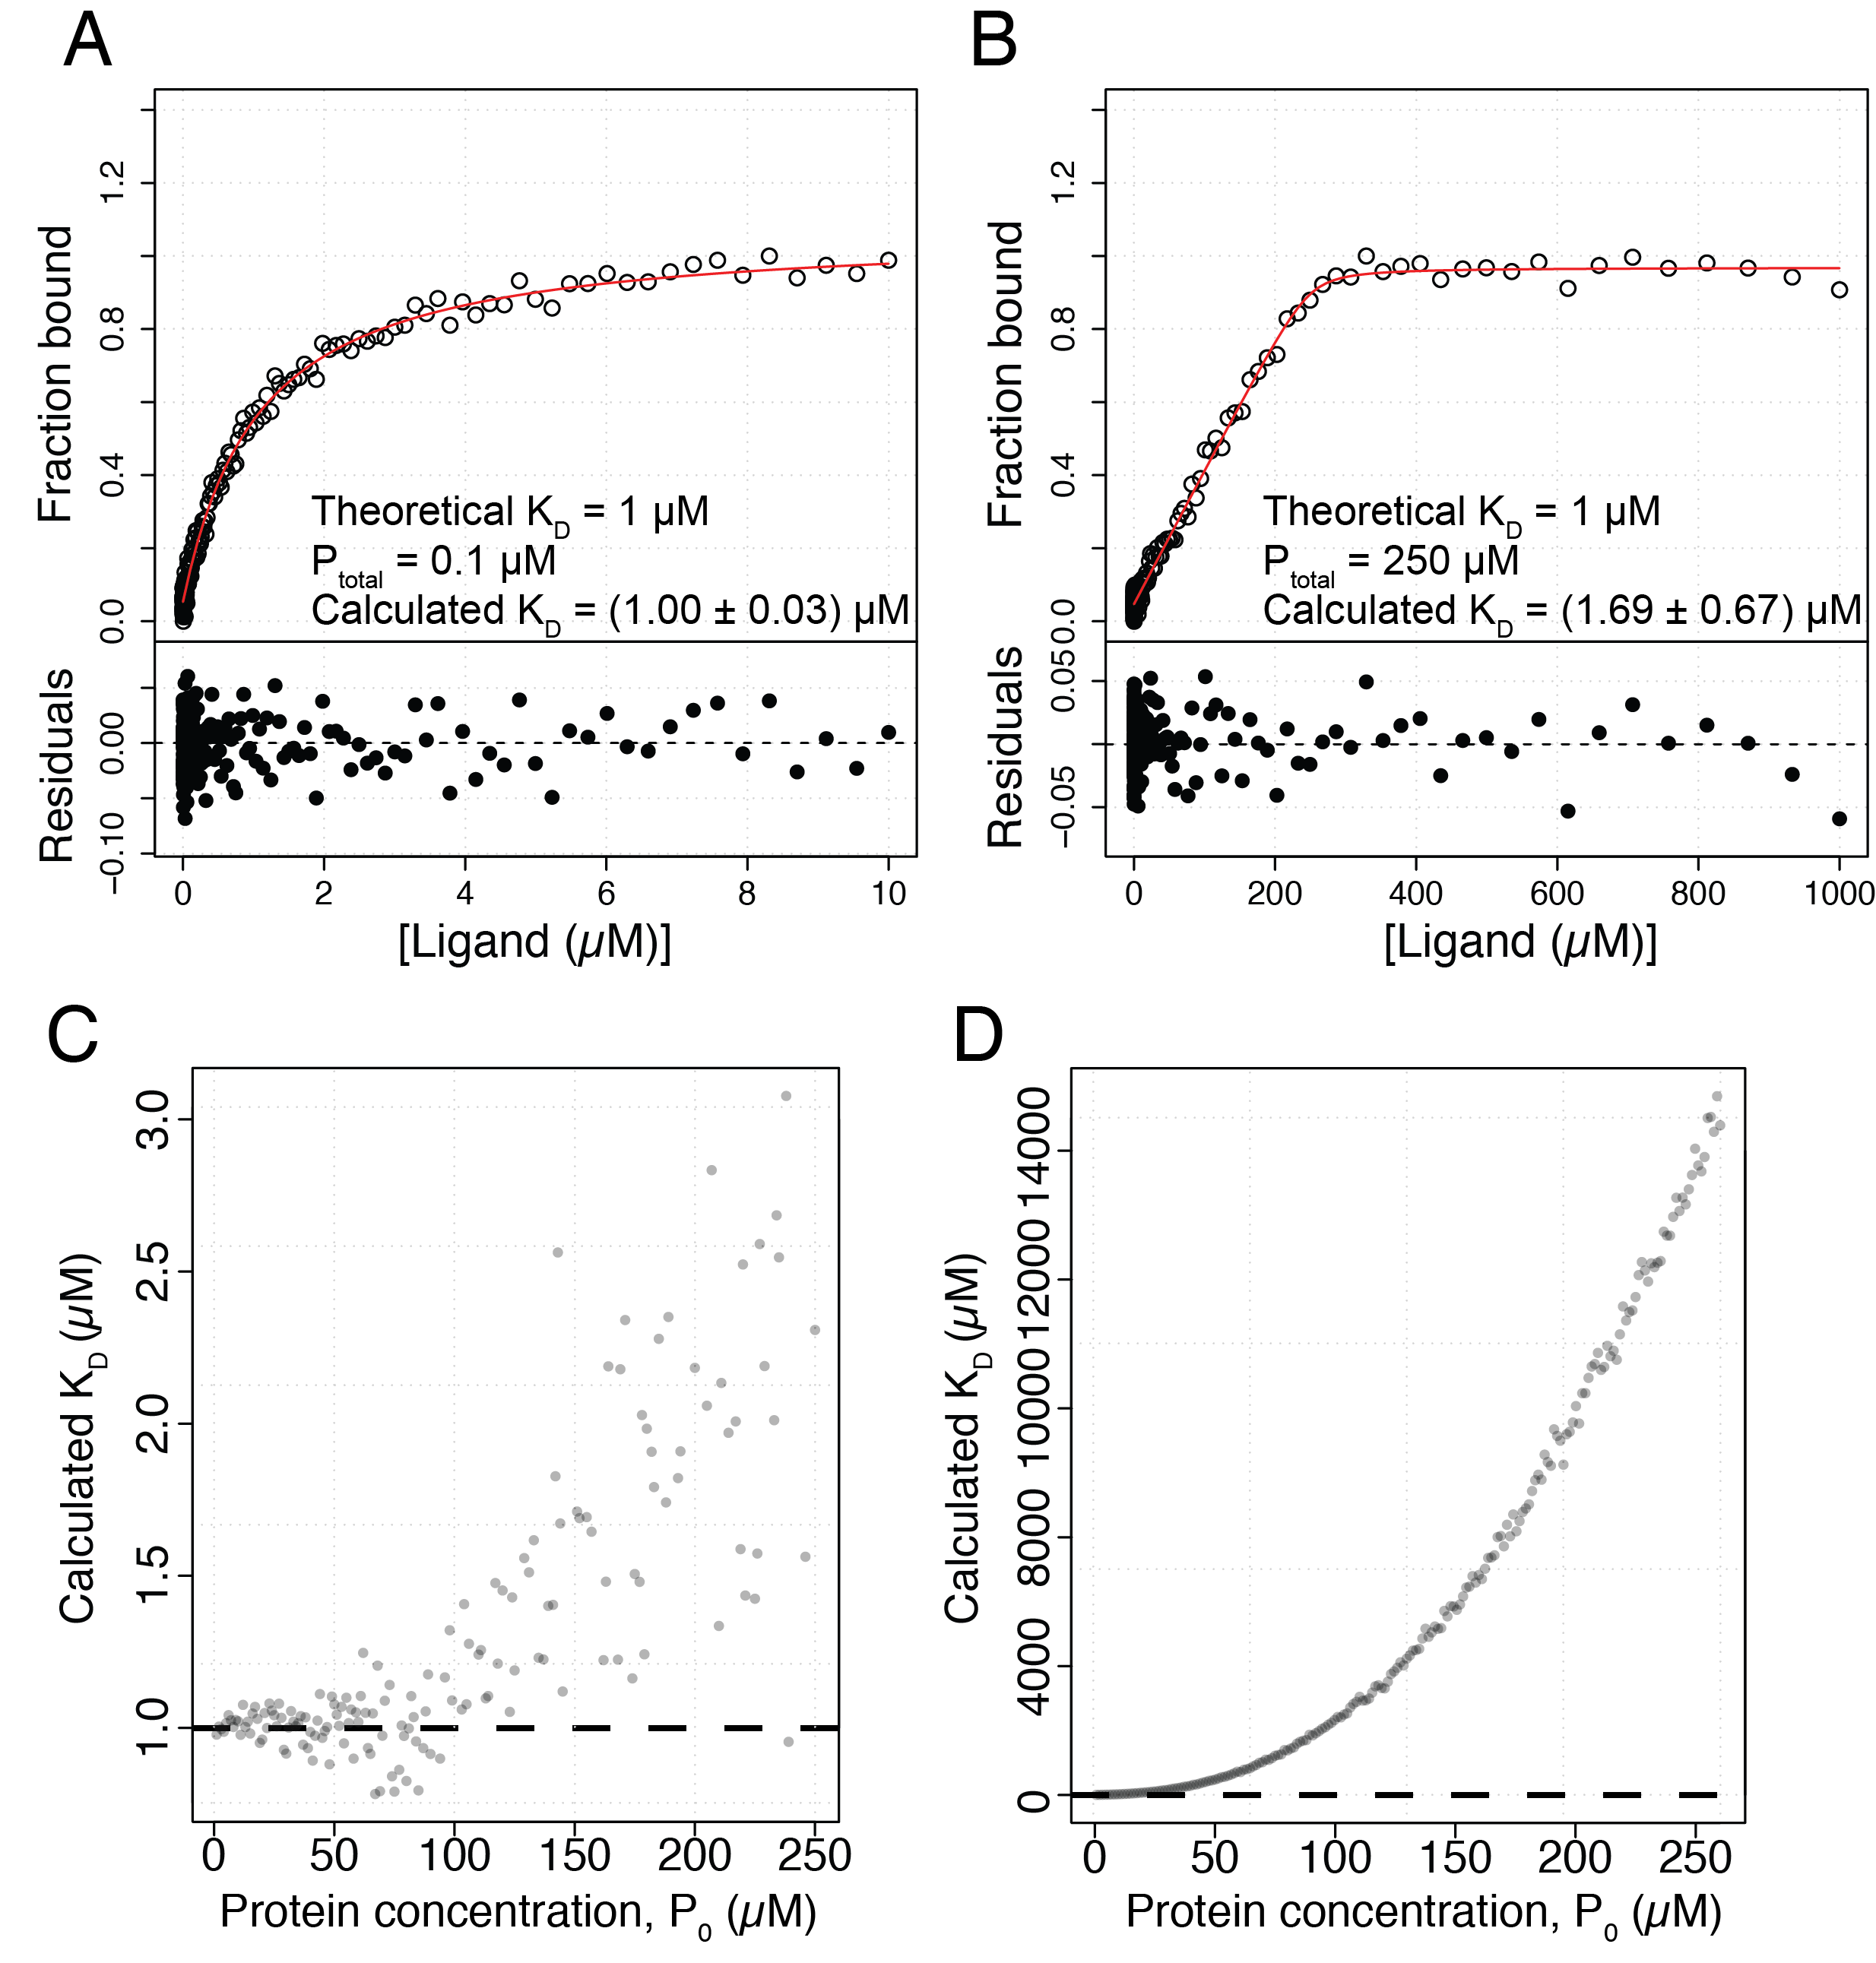
\includegraphics[scale=0.7]{ch4_fig2_binding_simulation.png}
\caption[Simulated protein-ligand binding data show that the measured binding affinity is over-estimated when high concentrations of protein are used in the experiment.] {\textbf{Simulated protein-ligand binding data show that the measured binding affinity is over-estimated when high concentrations of protein are used in the experiment.} \textbf{(A)} Binding data (open circles) were simulated with a defined theoretical $K_{D}$ of 1 $\mu$M and a protein concentration ($P_0$) of 0.1 $\mu$M (i.e $K_{D} >> P_{0}$). A binding curve was calculated from the simulated data (red curve), using the quadratic function $S_{obs}(S_{P}, S_{L}, S_{PL}, PL, K_{D})$ described in Equ. \ref{equ:mass_action}. \textbf{(B)} Binding data were simulated as in (A) with a defined theoretical $K_{D}$ of 1 $\mu$M and a protein concentration ($P_0$) of 250 $\mu$M (i.e $K_{D} << P_{0}$). \textbf{(C)} Binding affinities were calculated for simulated binding data with a theoretical KD = 1 $\mu$M over a range of $P_0$ concentrations, using the quadratic function $S_{obs}(S_{P}, S_{L}, S_{PL}, PL, K_{D})$ (Equ. \ref{equ:mass_action}) or \textbf{(D)} using the hyperbolic function $S_{obs}(K_{D})$ (Equ. \ref{equ:hill_equation}).}
\label{fig:binding_simulation}
\end{figure}
%
%
\clearpage



\subsection{FBP binding leads to an increase in the affinity of PKM2 for its substrate}
\label{subsec:pkm2activity_subs_affinity}
To investigate the mechanism of FBP-induced activation, steady-state kinetic parameters of PKM2 were determined in the presence and absence of FBP. In the absence of any added FBP, the $K_{M}^{PEP}$ was (1.22 $\pm$ 0.02) mM with a $k_{cat}$ of (349.3 $\pm$ 40.9) $s^{-1}$ (\textbf{Fig. \ref{fig:fbp_enzyme_activation} A} and \textbf{B}). Addition of saturating concentrations of FBP resulted in a six-fold reduction in the $K_{M}^{PEP}$ to (0.23 $\pm$ 0.04) mM, without a significant change in $k_{cat}$  (\textbf{Fig. \ref{fig:fbp_enzyme_activation} A} and \textbf{B}). The activation constant ($AC_{50}^{FBP}$) for FBP was measured as (118.1 $\pm$ 19.0) nM (\textbf{Fig. \ref{fig:fbp_enzyme_activation} C}), in excess of our previously measured $K_{D}^{FBP}$. Taken together, steady-state measurements of PKM2 catalysis suggested, consistent with previous findings, that FBP acts as a K-type activator to increase the binding affinity of the catalytic substrate PEP, without changing the rate of substrate turnover ($k_{cat}$).
%
%
%%% FIGURE
%
\begin{figure}[!ht]
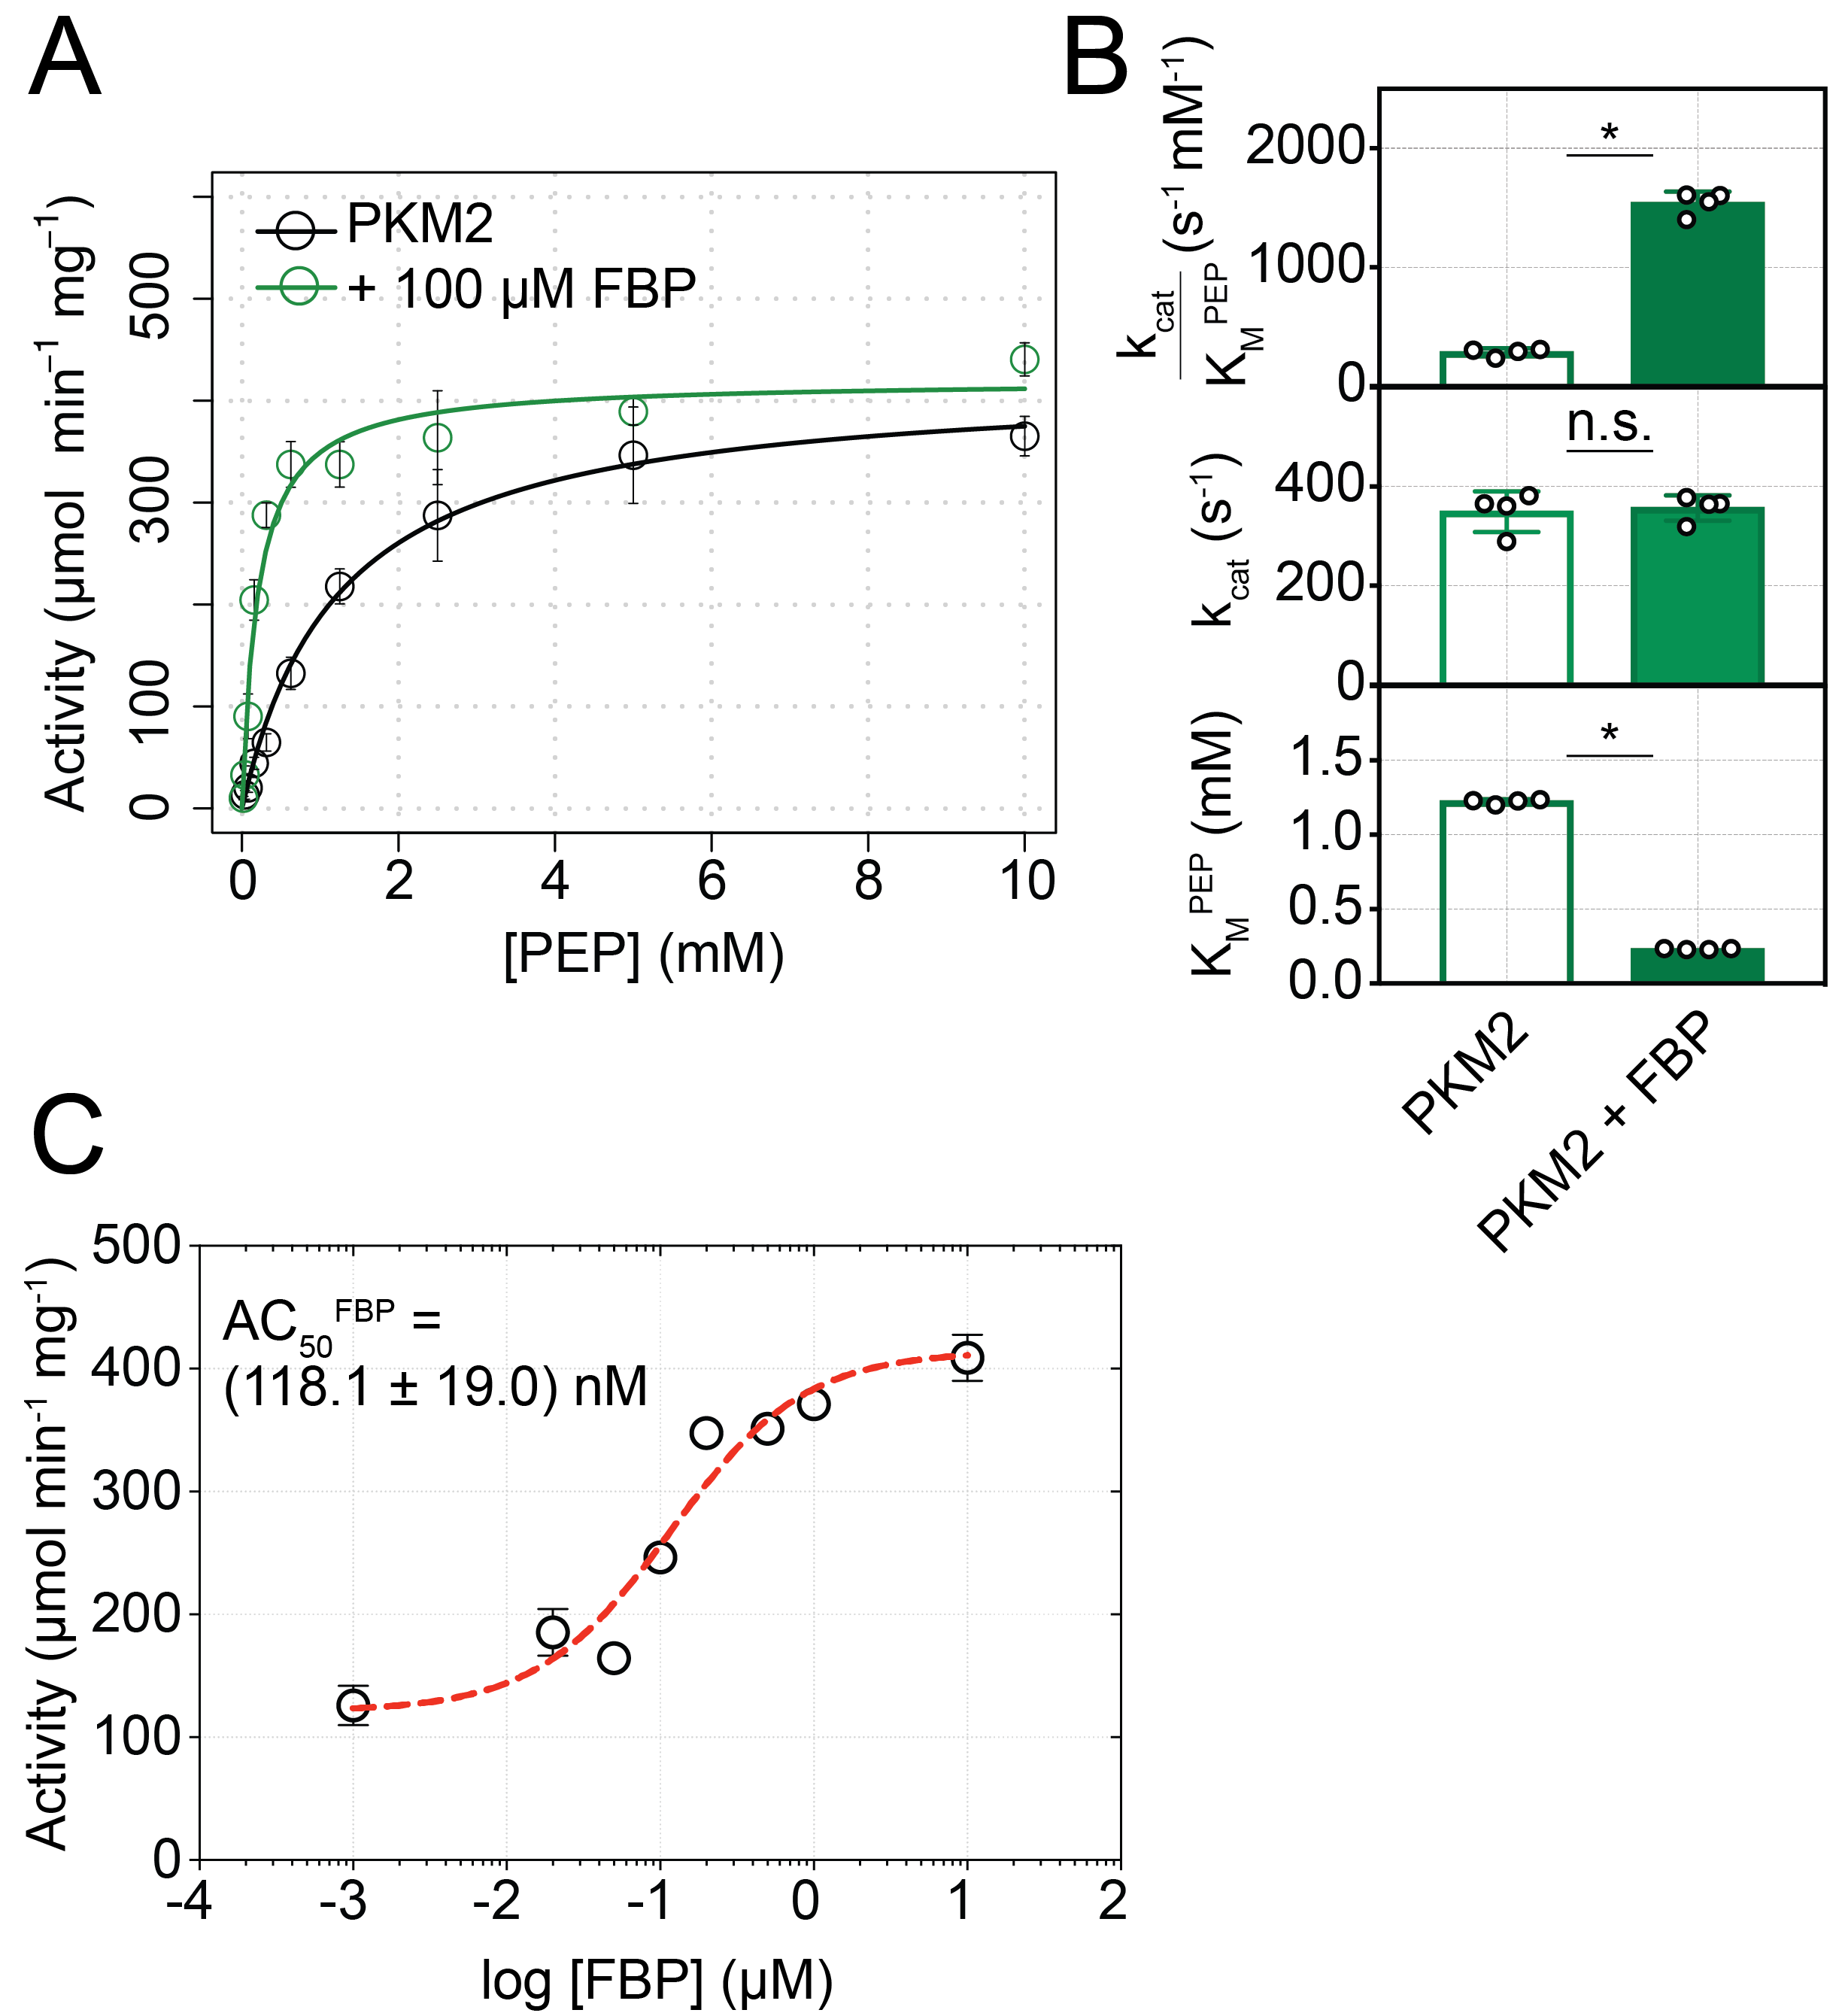
\includegraphics[scale=0.7]{ch4_fig3_pkm2activity.png}
\caption[Addition of FBP results in an increase in the substrate affinity of PKM2 for phosphoenolpyruvate.] {\textbf{Addition of FBP results in an increase in the substrate affinity of PKM2 for phosphoenolpyruvate.} \textbf{(A)} Specific activity of 5 nM PKM2 was measured using an LDH-coupled spectrophotometric assay (see Methods Section \ref{subsec:methods_pkm2_activity}) in the absence (black) and in the presence (green) of 2 $\mu$M added FBP. A constant concentration of 5 mM ADP was used, while varying the concentration of PEP. Measurements were performed at 37 \textdegree C. Rate curves were fitted using Michaelis-Menten kinetics. Means and standard deviations from four separate experiments are plotted. \textbf{(B)} Kinetic parameters were quantified from activity measurements of PKM2 in the absence (black) and in the presence (green) of 2 $\mu$M FBP. Significance was assessed using a Wilcoxon rank-sum test. Asterisk (*) marks significant changes (p-value < 0.05). \textbf{(C)} Specific activity of 5 nM PKM2 was measured at 1.5 mM PEP and 5 mM ADP, varying the concentration of FBP. A binding curve was fitted to the resulting rate curve assuming a 1:1 stoichiometry, to estimate the apparent activation constant ($AC_{50}^{FBP}$). Means and standard deviations of four separate experiments are plotted.}
\label{fig:fbp_enzyme_activation}
\end{figure}
%
%
\clearpage



\subsection{A phosphotyrosine peptide binds competitively with FBP to PKM2} \label{A phosphotyrosine peptide binds competitively with FBP to PKM2}
Given the finding that FBP binds to PKM2 with nano-molar affinity \textit{in vitro} (Section \ref{subsec:fbp_binding_pkm2}), consistent with previously reported $K_{D}^{FBP}$ measurements \cite{Gavriilidou:2018aa,Ikeda:1998aa,Yan:2016aa}, we sought to investigate possible mechanisms by which the affinity is reduced by competition with other ligands. Growth factor signalling mediated by phosphorylation of proteins at tyrosine residues, which is often upregulated in cancer, inhibits PKM2 activity by outcompeting FBP with a phosphotyrosine peptide motif \cite{Christofk:2008aa}. The mechanism of PKM2 phosphotyrosine peptide regulation, however, and the kinetics of its competition with FBP have not been characterised. We therefore sought to investigate the kinetics with which the phosphotyrosine peptide (M2tide) identified by Christofk \textit{et al.} (2008) \cite{Christofk:2008aa} displaces FBP.

\subsubsection{M2tide binds to PKM2 with an apparent affinity of 150 $\mu$M}
To this end, competition binding experiments between FBP and M2tide were performed by measuring the fluorescence anisotropy ($\lambda_{EX} = 494$ nm,  $\lambda_{EM} = 518$ nm) of a fluorescein-labelled M2tide variant (fluor-M2tide) \cite{Allali-Hassani:2009aa,Gao:2013aa}. \textcolor{red}{The sequence of fluor-M2tide is given: Fluorescein-GGAVDDD(PTyr)AQFANGG-COOH}.
%
%
\\\\
%
%
Preliminary experiments found that addition of PKM2 resulted in an increase in the anisotropy of fluor-M2tide (data not shown). Subsequent titrations of fluor-M2tide with PKM2 resulted in a concentration-dependent increase in the anisotropy of the peptide, which were used to calculate an apparent binding constant [$K_{D}^{fluor-M2tide}$ = (153 $\pm$ 19) $\mu$M] (\textbf{Fig. \ref{fig:peptide_binding} A}). Measurements were repeated with a single-point mutant PKM2(K433E), previously shown to disrupt phosphotyrosine binding to PKM2 \cite{Christofk:2008aa}. Consistent with this, we found that fluor-M2tide did not bind to PKM2(K433E), though a linear increase in the fluorescence anisotropy of the fluorescein probe was observed, likely a non-specific concentration-dependent effect of the labelled peptide (\textbf{Fig. \ref{fig:peptide_binding} B}). The notion that the linear fluorescence signal of the peptide arose from a non-specific effect, was supported by the observation that titrating the peptide with purified bovine serum albumin (BSA) resulted in a similar linear fluorescence anisotropic signal (\textbf{Fig. \ref{fig:peptide_binding} B}).

\subsubsection{M2tide and FBP competitively bind to PKM2}
To investigate the competitive binding kinetics between fluor-M2tide and FBP, fluorescence measurements of FBP-PKM2 binding were performed (as previously in Section \ref{subsec:fbp_binding_pkm2}) in the presence of increasing concentrations of fluor-M2tide. We found that addition of the peptide was accompanied by a linear increase the apparent $K_D^{FBP}$ (\textbf{Fig. \ref{fig:peptide_binding} C}), suggesting that the peptide and FBP competitively bind to PKM2. Conversely, while the K433E mutant abolished binding of fluor-M2tide, FBP binding was maintained albeit with a lower affinity [$K_D$ = (6.46 $\pm$ 1.46) $\mu$M] (\textbf{Fig. \ref{fig:peptide_binding} D}). Taken together, these results suggest that fluor-M2tide binds adjacent to the FBP pocket and that residue K433 provides a critical charged interaction for its binding, which would imply that the binding pockets for fluor-M2tide and FBP partially overlap.
%
%
%%% FIGURE
%
\begin{figure}[!ht]
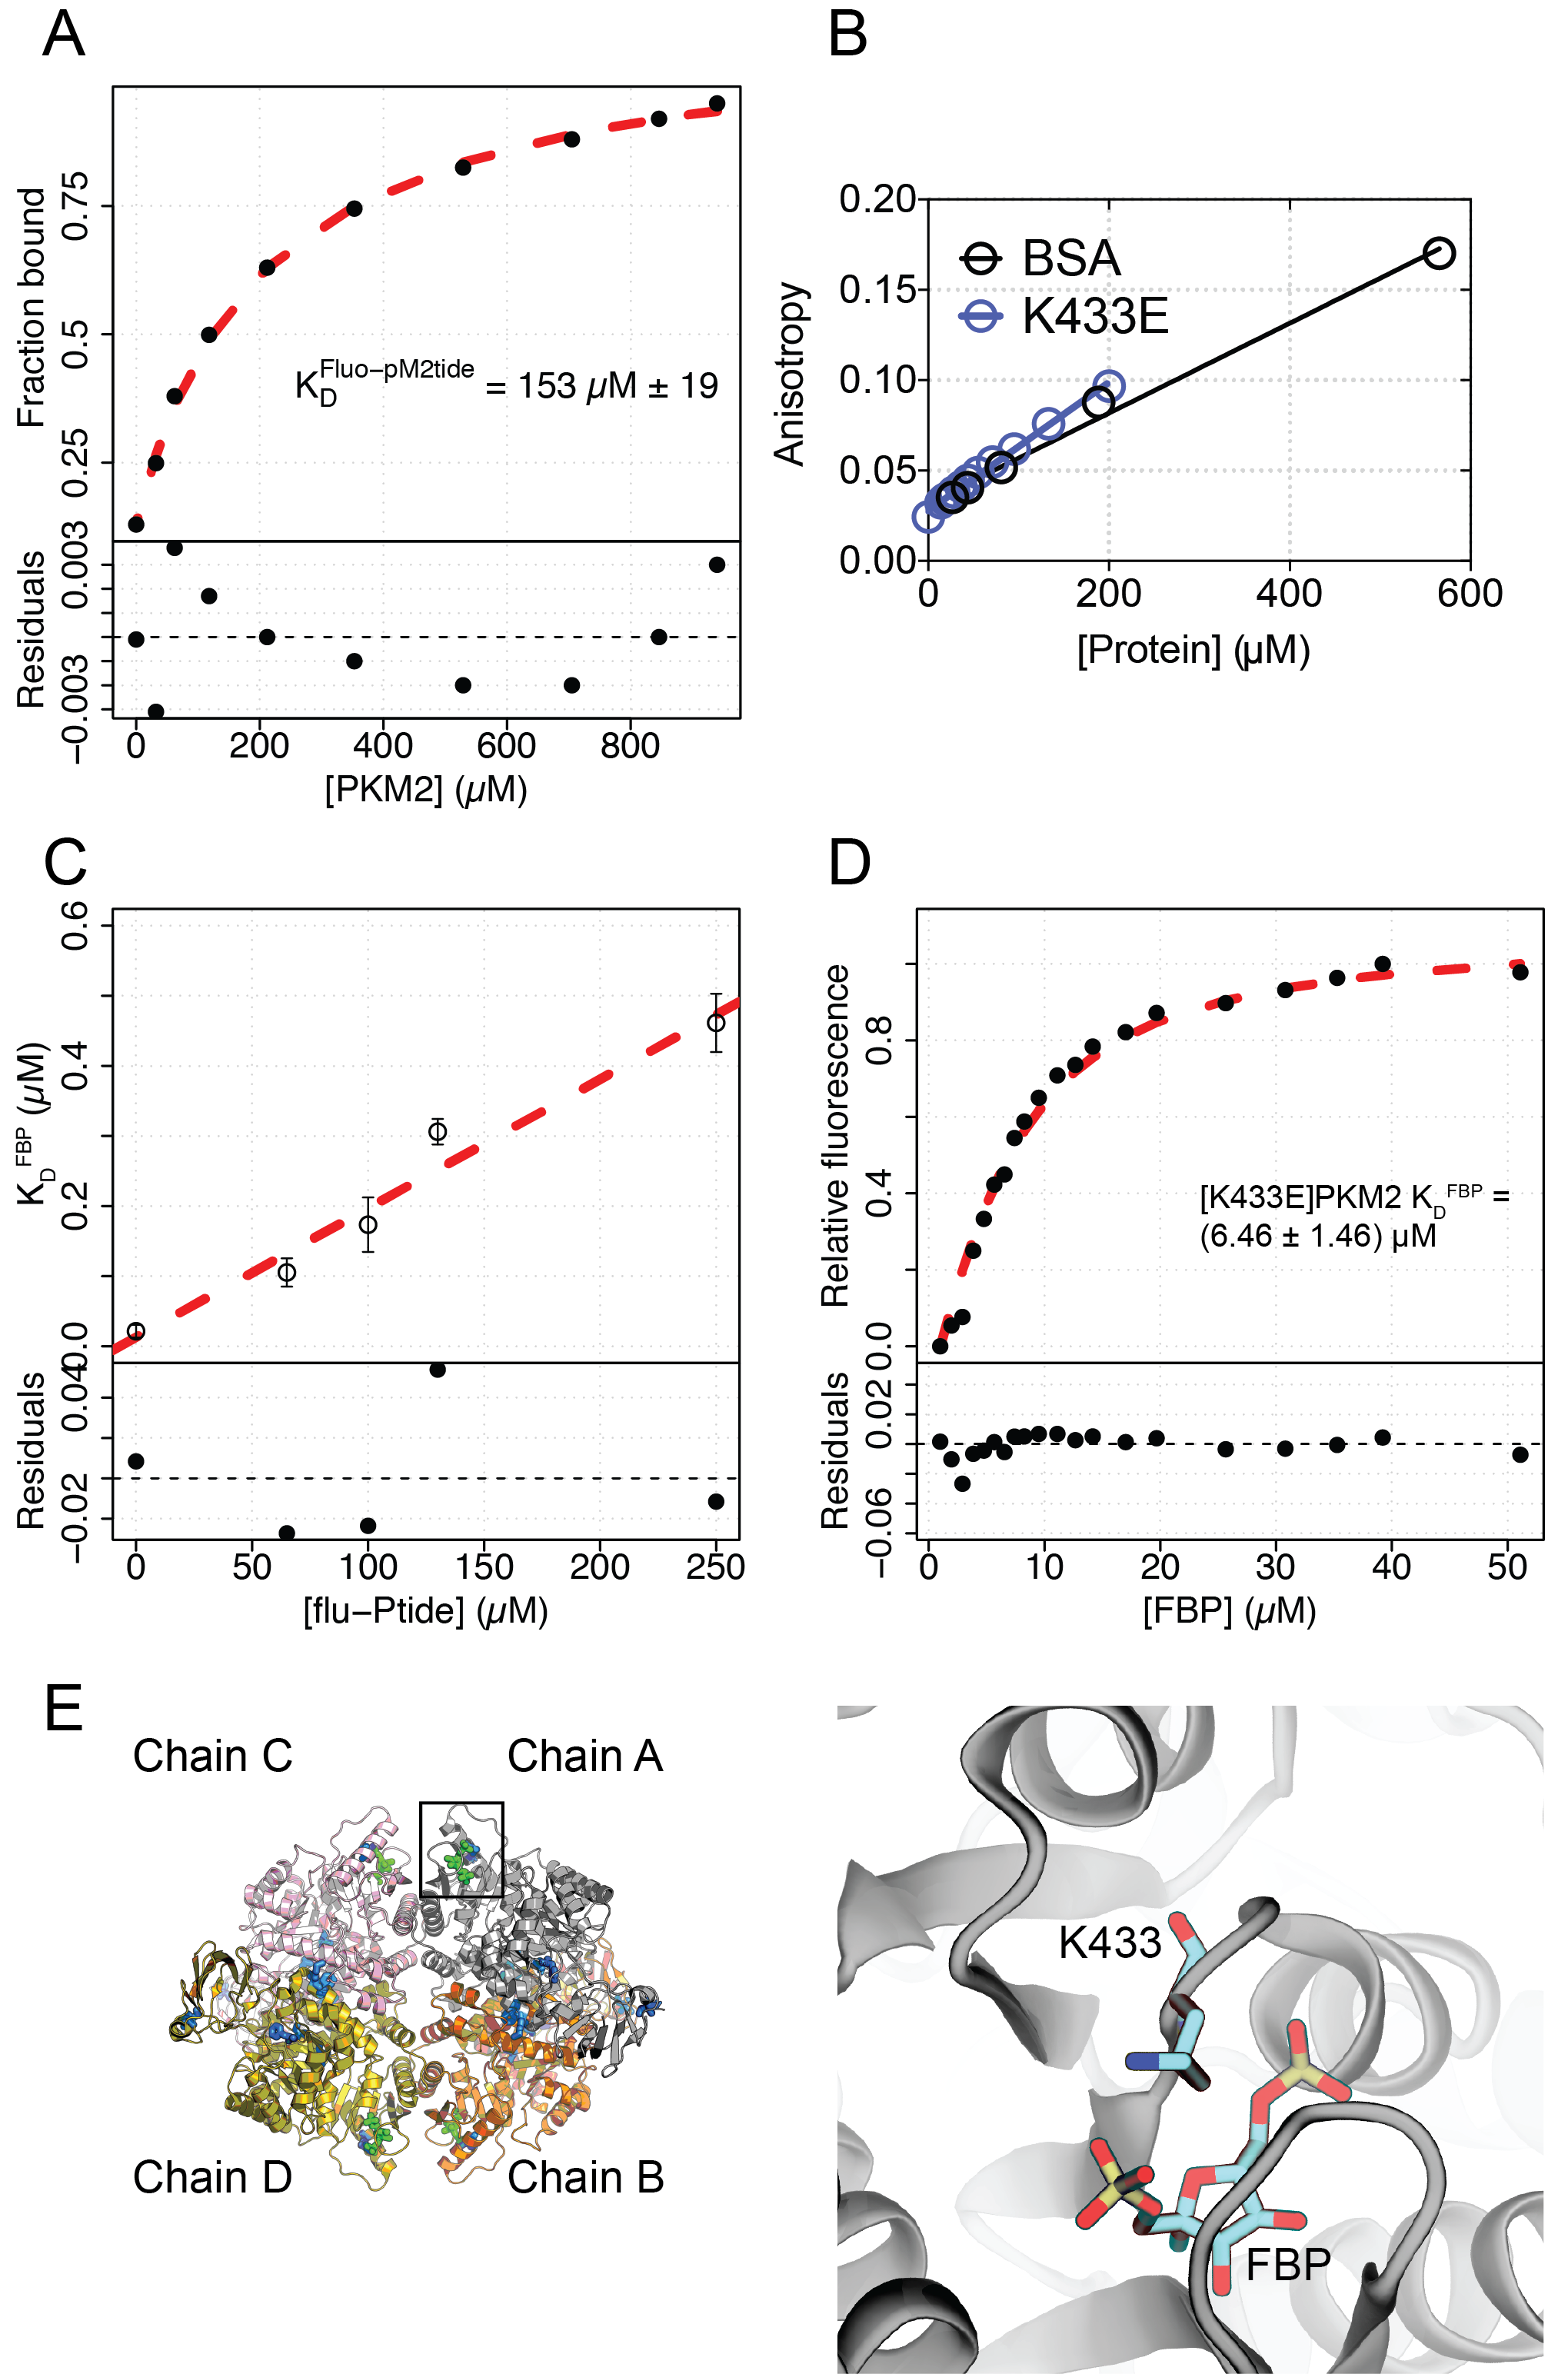
\includegraphics[scale=0.6]{ch4_fig4_peptide_binding.png}
\caption[Fluor-M2tide competes with FBP for binding to PKM2.] {\textbf{Fluor-M2tide competes with FBP for binding to PKM2.} \textbf{(A)} Fluorescence anisotropy measurements of a fluorescein-labelled peptide (fluor-M2tide) were performed at increasing concentrations of recombinant PKM2. The apparent binding affinity was estimated from a non-linear least squares regression of the binding curve. \textbf{(B)} Fluorescence anisotropy measurements of fluor-M2tide were acquired, titrating the concentrations of either PKM2(K433E) (blue) or bovine serum albumin (black). Anisotropy measurements were fitted with a linear regression. \textbf{(C)} Fluorescence emission measurements of PKM2 were performed to estimate the binding affinity of FBP at varying concentration of the fluor-M2tide peptide. Means and standard deviations from three independent titrations are plotted. \textbf{(D)} Fluorescence emission spectroscopy measurements of PKM2(K433E) were performed over a range of FBP concentrations. \textbf{(E)} A structural view of residue K433 relative to FBP bound in the crystal structure. Structural coordinates were extracted from the PDB accession code 3u2z.}
\label{fig:peptide_binding}
\end{figure}
%
%
\clearpage

\section{FBP binding to PKM2 induces inter-protomeric cooperativity}
Consistent with previous reports of FBP-induced activation of PKM2 \cite{Jurica:1998aa,Ikeda:1998aa,Dombrauckas:2005aa}, the previous Section found a K-type mechanism whereby FBP binding increases the effective affinity of the protein for the substrate phosphoenolpyruvate.  The reciprocal relationship between FBP binding and enzyme activation, however, is further complicated by the reported association of monomers and/or dimers into stable tetramers, which may invoke ligand-induced communication pathways between the four active sites in the tetramer forming the basis of inter-protomeric cooperativity. Alternatively, enzyme catalysis and subsequent activation of PKM2 protomers may act in isolation within the purported tetramer assembly.


\subsection{Titrating PKM2(WT) with the catalytically-dead PKM2(R72A) results in a non-linear decay in enzyme activity}
\label{subsec:exp_mutant_doping}

\subsubsection{A mutant-doping assay can be used to quantify inter-subunit cooperativity of a hetero-oligomeric protein}
In order to test the hypothesis that FBP-induced allosteric activation promotes inter-subunit co-operativity, we sought to monitor the kinetics in the decay of PKM2 activity as PKM2(WT) was titrated with a catalytically-inactive mutant variant of PKM2, in a so-called \textit{mutant doping} assay \cite{Moreau:2007aa,Rzechorzek:2014aa,Barry:2009aa,Crampton:2006aa}. In this assay, PKM2(WT) was titrated with a catalytically-inactive mutant variant of PKM2 to form hetero-oligomeric species with defined stoichiometric ratios of WT subunits and inactive subunits. The enzyme activity of each mixture is measured, which decreases with increasing concentrations of the inactive species in the mixture. For proteins with a cooperative dependence on the adjacent subunits in an oligomeric assembly, the decrease in activity is non-linear. Conversely, for proteins where the subunits function independently of their neighbouring subunits within an oligomeric assembly, the activity decay is linear. Therefore, the inter-subunit of an oligomeric protein can be quantified by fitting the decay in enzyme activity as the WT protein is \textit{doped} with an inactive variant. 

\subsubsection{PKM2(R72A) is inactive and hetero-oligomerises with PKM2(WT)}
To first identify a single-point mutant that depleted PK phosphotransferase activity, the enzyme activity of three active site mutants [PKM2(R72A), PKM2(R120A) and PKM2(K270A)] were measured. Initial velocity curves revealed that, compared to PKM2(WT) [$k_{cat} = (538.4 \pm 18.0) \: s^{-1}$] the rate of product turnover was decreased by approximately 1.7-fold for PKM2(R120) [$k_{cat} = (308.4 \pm 5.7) \: s^{-1}$] and PKM2(K270A) [$k_{cat} = (270.8 \pm 5.3) \: s^{-1}$] (\textbf{Fig. \ref{fig:mut_doping_exp} A}). Moreover, activity of PKM2(R72A) was almost entirely abolished, evidenced by a 63-fold decrease in the apparent rate of substrate turnover [$k_{cat} = (8.5 \pm 1.4) \: s^{-1}$] (\textbf{Fig. \ref{fig:mut_doping_exp} A}). 
%
%
\\\\
%
%
To measure the inactivating effect of introducing catalytically inactive protomeric units into a hetero-oligomeric assembly with PKM2(WT), it was first necessary to establish that PKM2(R72A) did not disrupt oligomerisation. First, microscale thermophoresis (MST) measurements of fluorescein-labelled PKM2(WT) were performed with titrated amounts of unlabelled PKM2(WT), to measure PKM2(WT) oligomeric association. A concentration-dependent change in PKM2 thermophoresis was detected, from which an apparent oligomerisation constant ($K_{D}^{oligo}$) of (90.8 $\pm$ 5.7) nM was estimated for PKM2(WT) (Table \ref{tab:oligo_kds}). The apparent oligomerisation constant of PKM2(WT) was found to be unchanged upon addition of saturating concentrations of FBP, yielding a $K_{D}^{oligo}$ of (97.9 $\pm$ 1.8) nM (Table \ref{tab:oligo_kds}).
%
%
\\\\
%
%
MST measurements of labelled-PKM2(WT) were repeated with titrated amounts of PKM2(R72A), revealing a 4-fold increase in the $K_{D}^{oligo}$ both in the absence [(410 $\pm$ 20) nM] and presence [(390 $\pm$ 40) nM] of saturating concentrations of FBP (\textbf{Fig. \ref{fig:mut_doping_exp} B}) and \textbf{Table \ref{tab:oligo_kds}}). Despite the reduction in the apparent $K_{D}^{oligo}$ for [WT]PKM2 and PKM2(R72A) association, a similar maximal thermophoretic behaviour of the labelled-PKM2(WT) at high concentrations of the mutant suggested that the catalytically-dead variant formed hetero-oligomeric assemblies with the wild-type, albeit with marginally weaker binding. 
%
%
%%% TABLE
% Please add the following required packages to your document preamble:
% \usepackage{booktabs}
\begin{table}[h]
\centering
\caption[Dissociation constants for PKM2 self-association and hetero-association with PKM2(R72A), under various liganded conditions.]{\textbf{Dissociation constants for PKM2 self-association and hetero-association with PKM2(R72A), under various liganded conditions.} All measurements were made by titrating fluorscein-labelled PKM2(WT) with either unlablled PKM2(WT) or unlabelled PKM2(R72A).}
\label{tab:oligo_kds}
\begin{tabular}{@{}lll@{}}
\toprule
Titrant        & Ligands          & $K_{D}^{oligo}$ (nM) \\ \midrule
PKM2(WT)   & None             & 90.8 $\pm$ 5.7            \\
PKM2(WT)   & 2 $\mu$M FBP     & 97.9 $\pm$ 1.8            \\
PKM2(WT)   & 2 $\mu$M Tepp-46 & 54.6 $\pm$ 2.1            \\
PKM2(WT)   & 5 mM ADP         & 75.8 $\pm$ 6.4            \\
PKM2(WT)   & 10 mM PEP        & 52.1 $\pm$ 10.1           \\
PKM2(R72A) & None             & 410.0 $\pm$ 20.0          \\
PKM2(R72A) & 2 $\mu$M FBP     & 390.0 $\pm$ 40.0          \\ \bottomrule
\end{tabular}
\end{table}
%
%
%
\subsubsection{Titration of PKM2(WT) with PKM2(R72A) results in a non-linear decay in enzyme activity}
Next, the mutant doping assay was performed whereby stoichiometric mixtures of PKM2(R72A) and PKM2(WT) were assayed for pyruvate kinase activity. PKM2(WT)-PKM2(R72A) mixtures were prepared at a total protein concentration of 5 $\mu$M, an order of magnitude in excess of the measured $K_{D}^{oligo}$, thereby circumventing the reduced affinity of the mutant for the wild-type. A linear decay in activity was observed over a range of substrate concentrations, with increasing $\frac{[PKM2(R72A)]}{[PKM2(WT)]}$, in the absence of added FBP (\textbf{Fig. \ref{fig:mut_doping_exp} C}). Conversely, addition of saturating concentrations of FBP resulted in a non-linear decay in enzyme activity of the $\frac{[PKM2(R72A)]}{[PKM2(WT)]}$ mixtures (\textbf{Fig. \ref{fig:mut_doping_exp} D}), suggesting an FBP-induced cooperative effect between the PKM2 subunits.
%
%
%%% FIGURE
%
\begin{figure}[!ht]
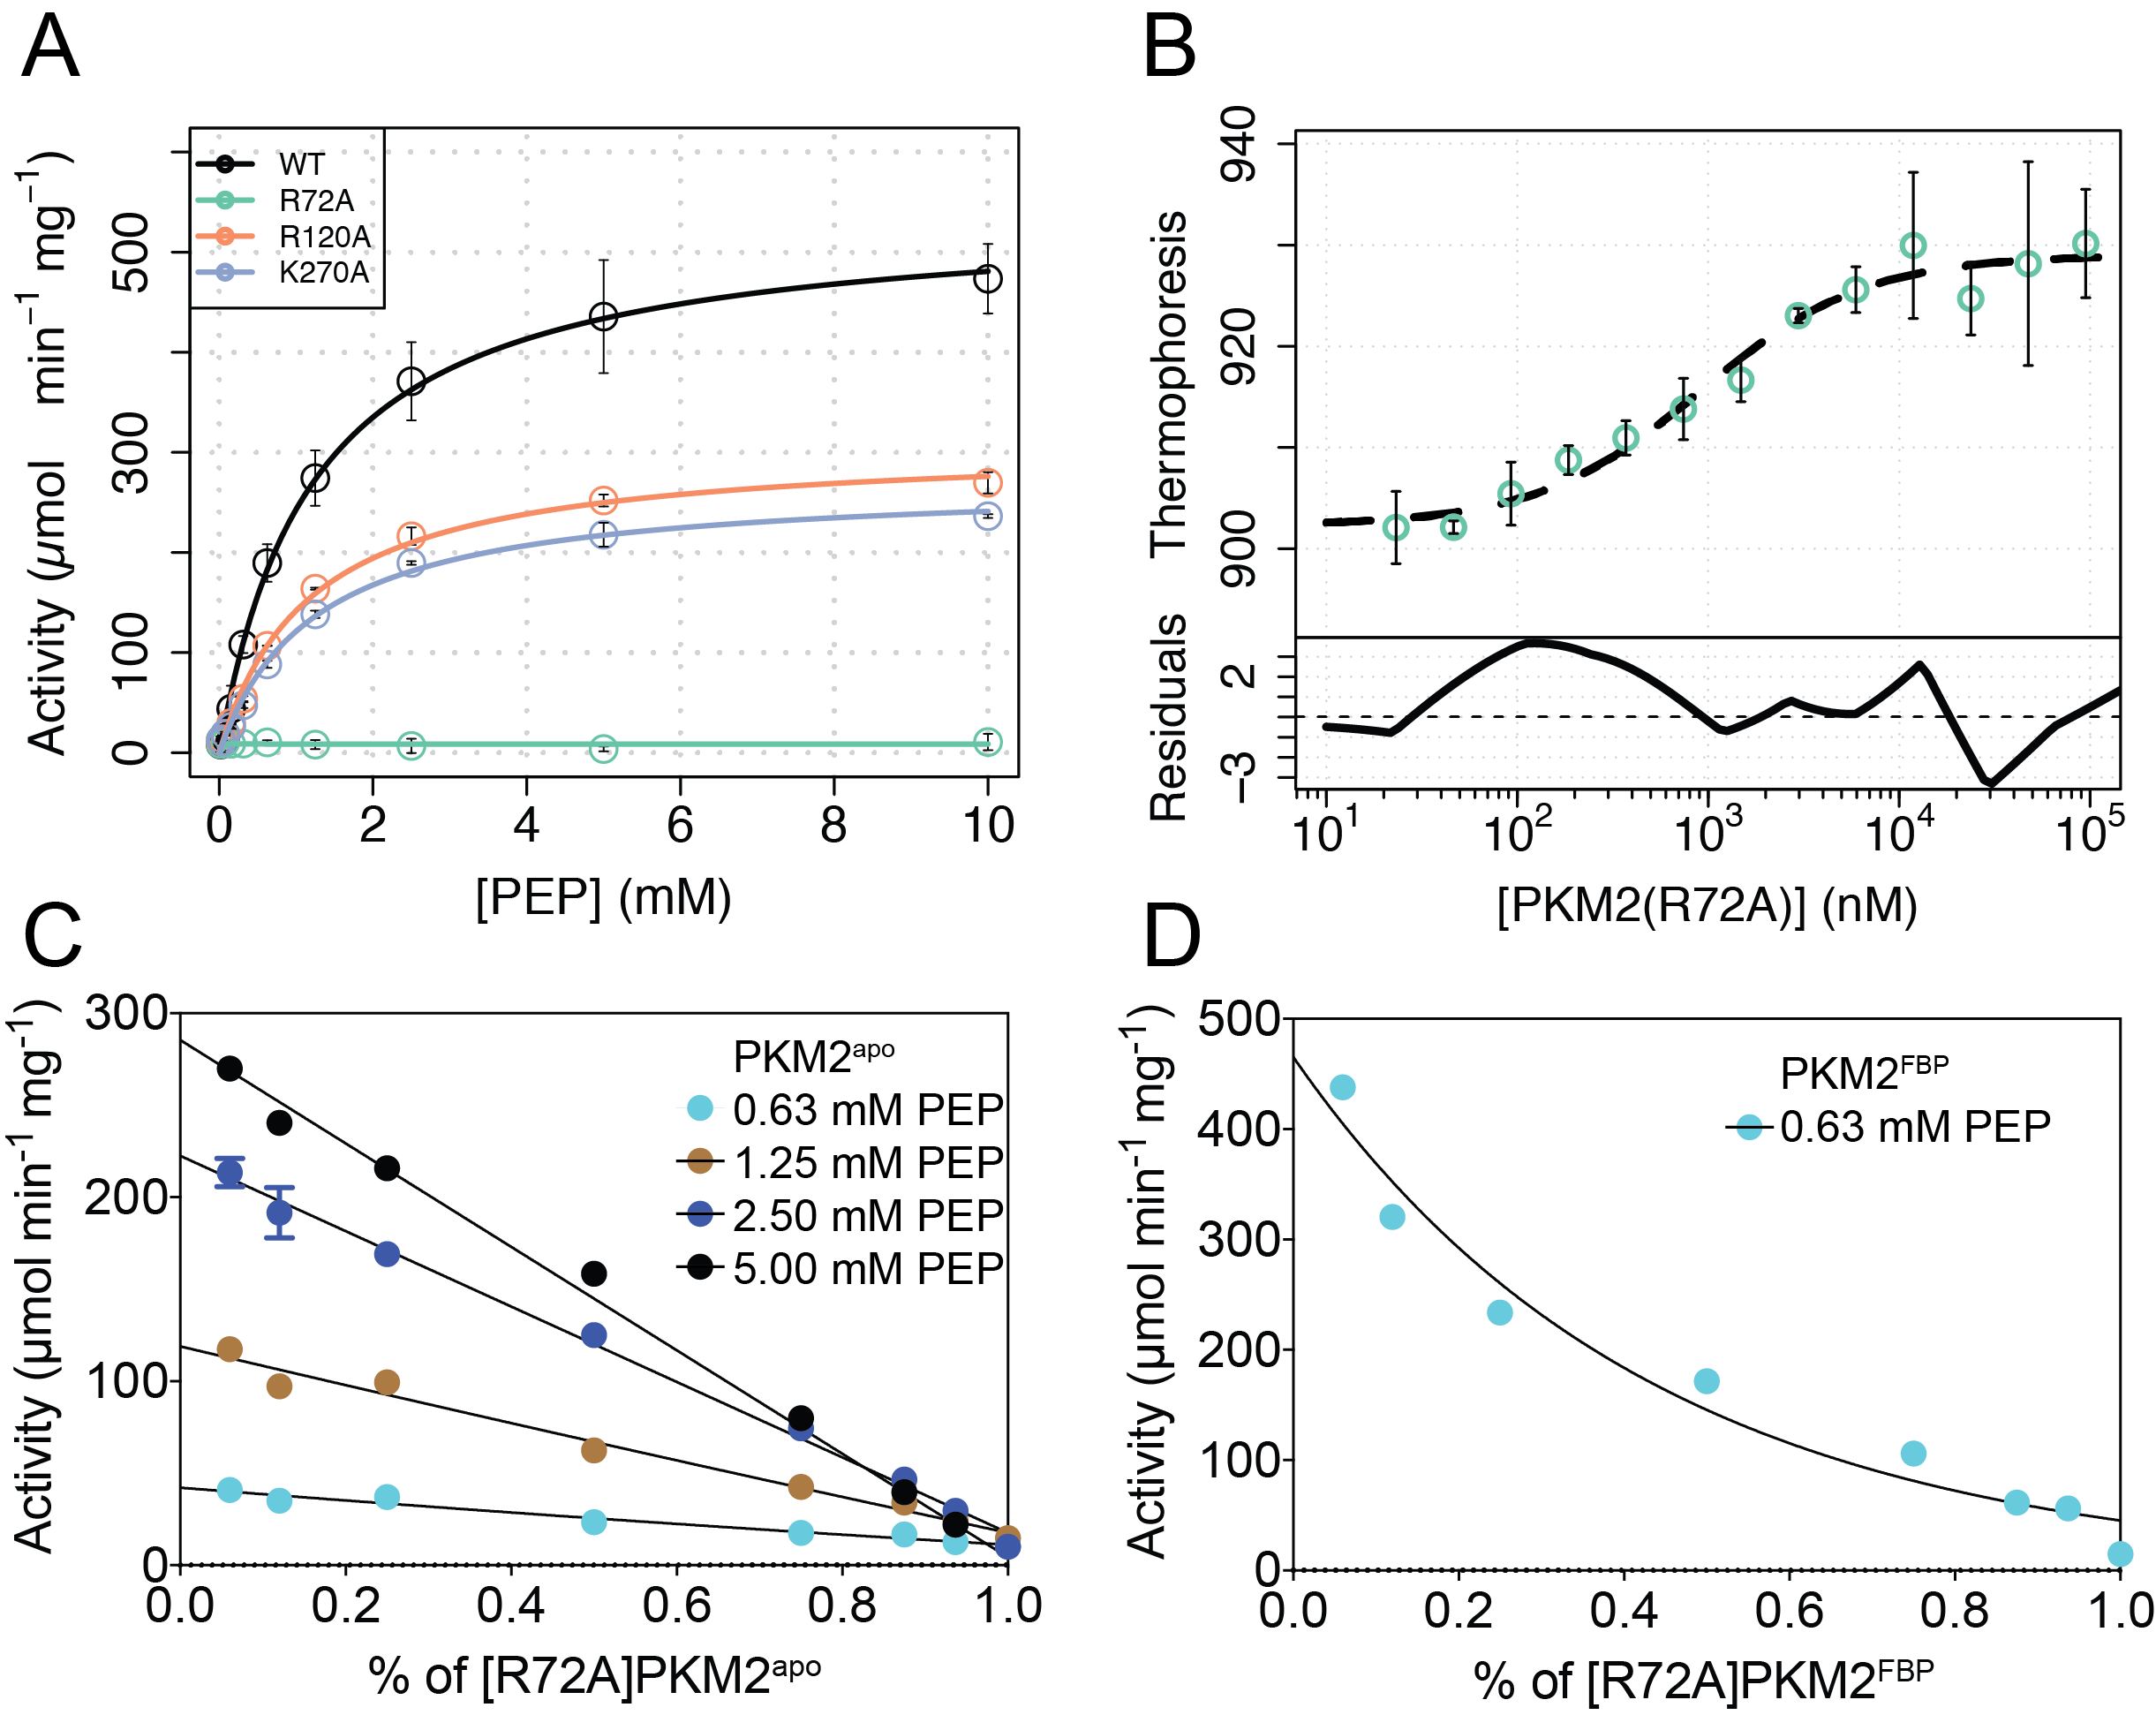
\includegraphics[scale=0.7]{ch4_fig8_mutant_doping_exp.png}
\caption[A mixture of wild-type and catalytically-dead PKM2 has a non-linear decay in activity.] {\textbf{A mixture of wild-type and catalytically-dead PKM2 has a non-linear decay in activity.} \textbf{(A)} Initial velocity measurements were recorded over a range of PEP concentrations at a constant concentration of 5 mM ADP at 310 \textdegree C for PKM2(WT) (black) and active-site mutant variants PKM2(R72A) (teal), PKM2(R120A) (orange) and PKM2(K270A) (blue). The mean and standard deviation of four separate experiments are shown, for each protein variant. Kinetic parameters were estimated from Michaelis-Menten fits of the rate curves. \textbf{(B)} Microscale thermophoresis measurements were acquired for titrations of fluorescein-labelled PKM2(WT) with PKM2(R72A). \textbf{(C)} Mixtures of PKM2(WT) with PKM2(R72A) were assayed for enzyme activity over a range of substrate concentrations in the absence and \textbf{(D)} in the presence of 2 $\mu$M FBP.}
\label{fig:mut_doping_exp}
\end{figure}
%
%
\clearpage

\subsection{A numerical framework for modelling oligomeric enzyme cooperativity}
The non-linear decay in enzyme activity of mutant-doped PKM2, upon FBP addition (Section \ref{subsec:exp_mutant_doping}), suggested a ligand-dependent inter-subunit cooperativity. To rationalise this observation, a numerical framework was constructed whereby the inter-subunit cooperativity of a tetrameric protein could be simulated, and compared to experimental data.
%
%
\\\\
%
%
To this end, a model was generated to consider the enzyme activity resulting from the mixture of active PKM2(WT) oligomers (\textit{A}) and inactive PKM2(R72A) (\textit{I}) oligomers. We assumed that the measured association between PKM2(WT) and PKM2(R72A) formed tetramers and that the composition of the tetramers was purely stochastic. Moreover, it was posited that the mixture of \textit{A} and \textit{I} was defined by the ratio of the concentrations of \textit{A} and \textit{I}. 
%
%
\\\\
%
%
Given the above assumptions, five configurations of hetero-tetramers resulting from the mixture of PKM2(WT) and PKM2(R72A) are possible, not counting permutations under the assumption of a stochastic association: AAAA, AAAI, AAII, AIII, IIII. The concentration of \textit{A} is given by \textit{a} and the concentration of \textit{I} is given by \textit{i}. Therefore the ratio between \textit{A} and \textit{I} is:
%
\begin{equation}
r = \frac{a}{i}
\end{equation}
%
The total concentration is trivially given by:
%
\begin{equation}
C = a + i
\end{equation}
%
%
A final assumption made in this model was that the enzyme activity of \textit{A} is 1 AU (\textit{activity unit}) and that the corresponding activity of \textit{I} is equal to 0 AU. Additionally, under conditions where \textit{A} and \textit{I} catalytic sites function in complete isolation (\textit{ie.} no inter-subunit cooperativity), the enzyme activity (\textit{ea}) of the mixtures are given by the following expression:
%
%
\begin{equation}
ea(AAAA) = \frac{4}{3} \cdot ea(AAAI) = 2 \cdot ea(AAII) =4 \cdot ea(AIII)
\end{equation}
%
%
\begin{equation}
ea = \sum_{n=1}^{4} n(A+I) 
\end{equation}
%
%
From this, the probability of observing a fully active tetrameric species from a sequential mixture of \textit{a} and \textit{i} is given by a binomial distribution:
%
\begin{equation}
P(A) = \left[ \binom{n}{A} a^{A} (1-a)^{n-A} \right]^{AC}
\label{equ:bin_mix_model}
\end{equation}
%
%
where \textit{AC} is the allosteric coefficient, an added exponential term, defined by the strength of inter-protomeric cooperativity between individual subunits in the tetramer assembly (\textbf{Fig. \ref{fig:mut_doping_theory} A}).
%
%
\\\\
%
%
The mixture model in Equ. \ref{equ:bin_mix_model} was simulated over a range of increasing values of $AC$. Where $AC = 1$, a linear decrease in activity was observed (\textbf{Fig. \ref{fig:mut_doping_theory} B}). Conversely, where $AC > 1$ a non-linear decay in activity of the model was observed (\textbf{Fig. \ref{fig:mut_doping_theory} C}). The magnitude of the non-linear decrease in activity was found to be enhanced, with greater pre-defined values for \textit{AC} (\textbf{Fig. \ref{fig:mut_doping_theory} C}). 


\subsection{FBP binding induced inter-subunit cooperativity under conditions of limiting substrate concentrations}
The mixture model of enzyme activity was applied towards analysing initial velocity measurements resulting from ratio-metric mixtures of PKM2(WT) and PKM2(R72) by performing a non-linear regression of the activity data to Equ. \ref{equ:bin_mix_model}. Solutions for the allosteric coefficient ($AC$) were computed using a non-linear least squares procedure, as a means of quantifying the strength of inter-protomeric cooperativity within hetero-oligomeric assemblies of PKM2. 
%
%
\\\\
%
%
The linear decay in enzyme activity, in the absence of any added FBP, supported the hypothesis that protomers within PKM2 oligomers were acting largely in isolation, with no detectable cooperativity between the individual catalytic pockets. This expectation was reflected in the solution to the $AC$, which was found to be $\simeq 1$ (\textbf{Fig. \ref{fig:mut_doping_theory} D}). In contrast, the observed non-linear decay in enzyme activity, upon addition of saturating concentrations of FBP resulted in an increase in the solution for the allosteric coefficient. Moreover, this non-linear effect, and as such the allosteric coefficient strength, was found to increase at concentrations of substrate below the $K_{M}^{PEP}$ (\textbf{Fig. \ref{fig:mut_doping_theory} D}). The correlation of the $AC$ with the concentration of phosphoenolpyruvate suggested a mechanism whereby FBP binding acts to increase the cooperativity between individual subunits under conditions where the substrate is limiting. Conversely, when the substrate concentrations are near-saturating, FBP-induced inter-subunit cooperativity is diminished, regulate the activity of PKM2.
%
%
%
%%% FIGURE
%
\begin{figure}[!ht]
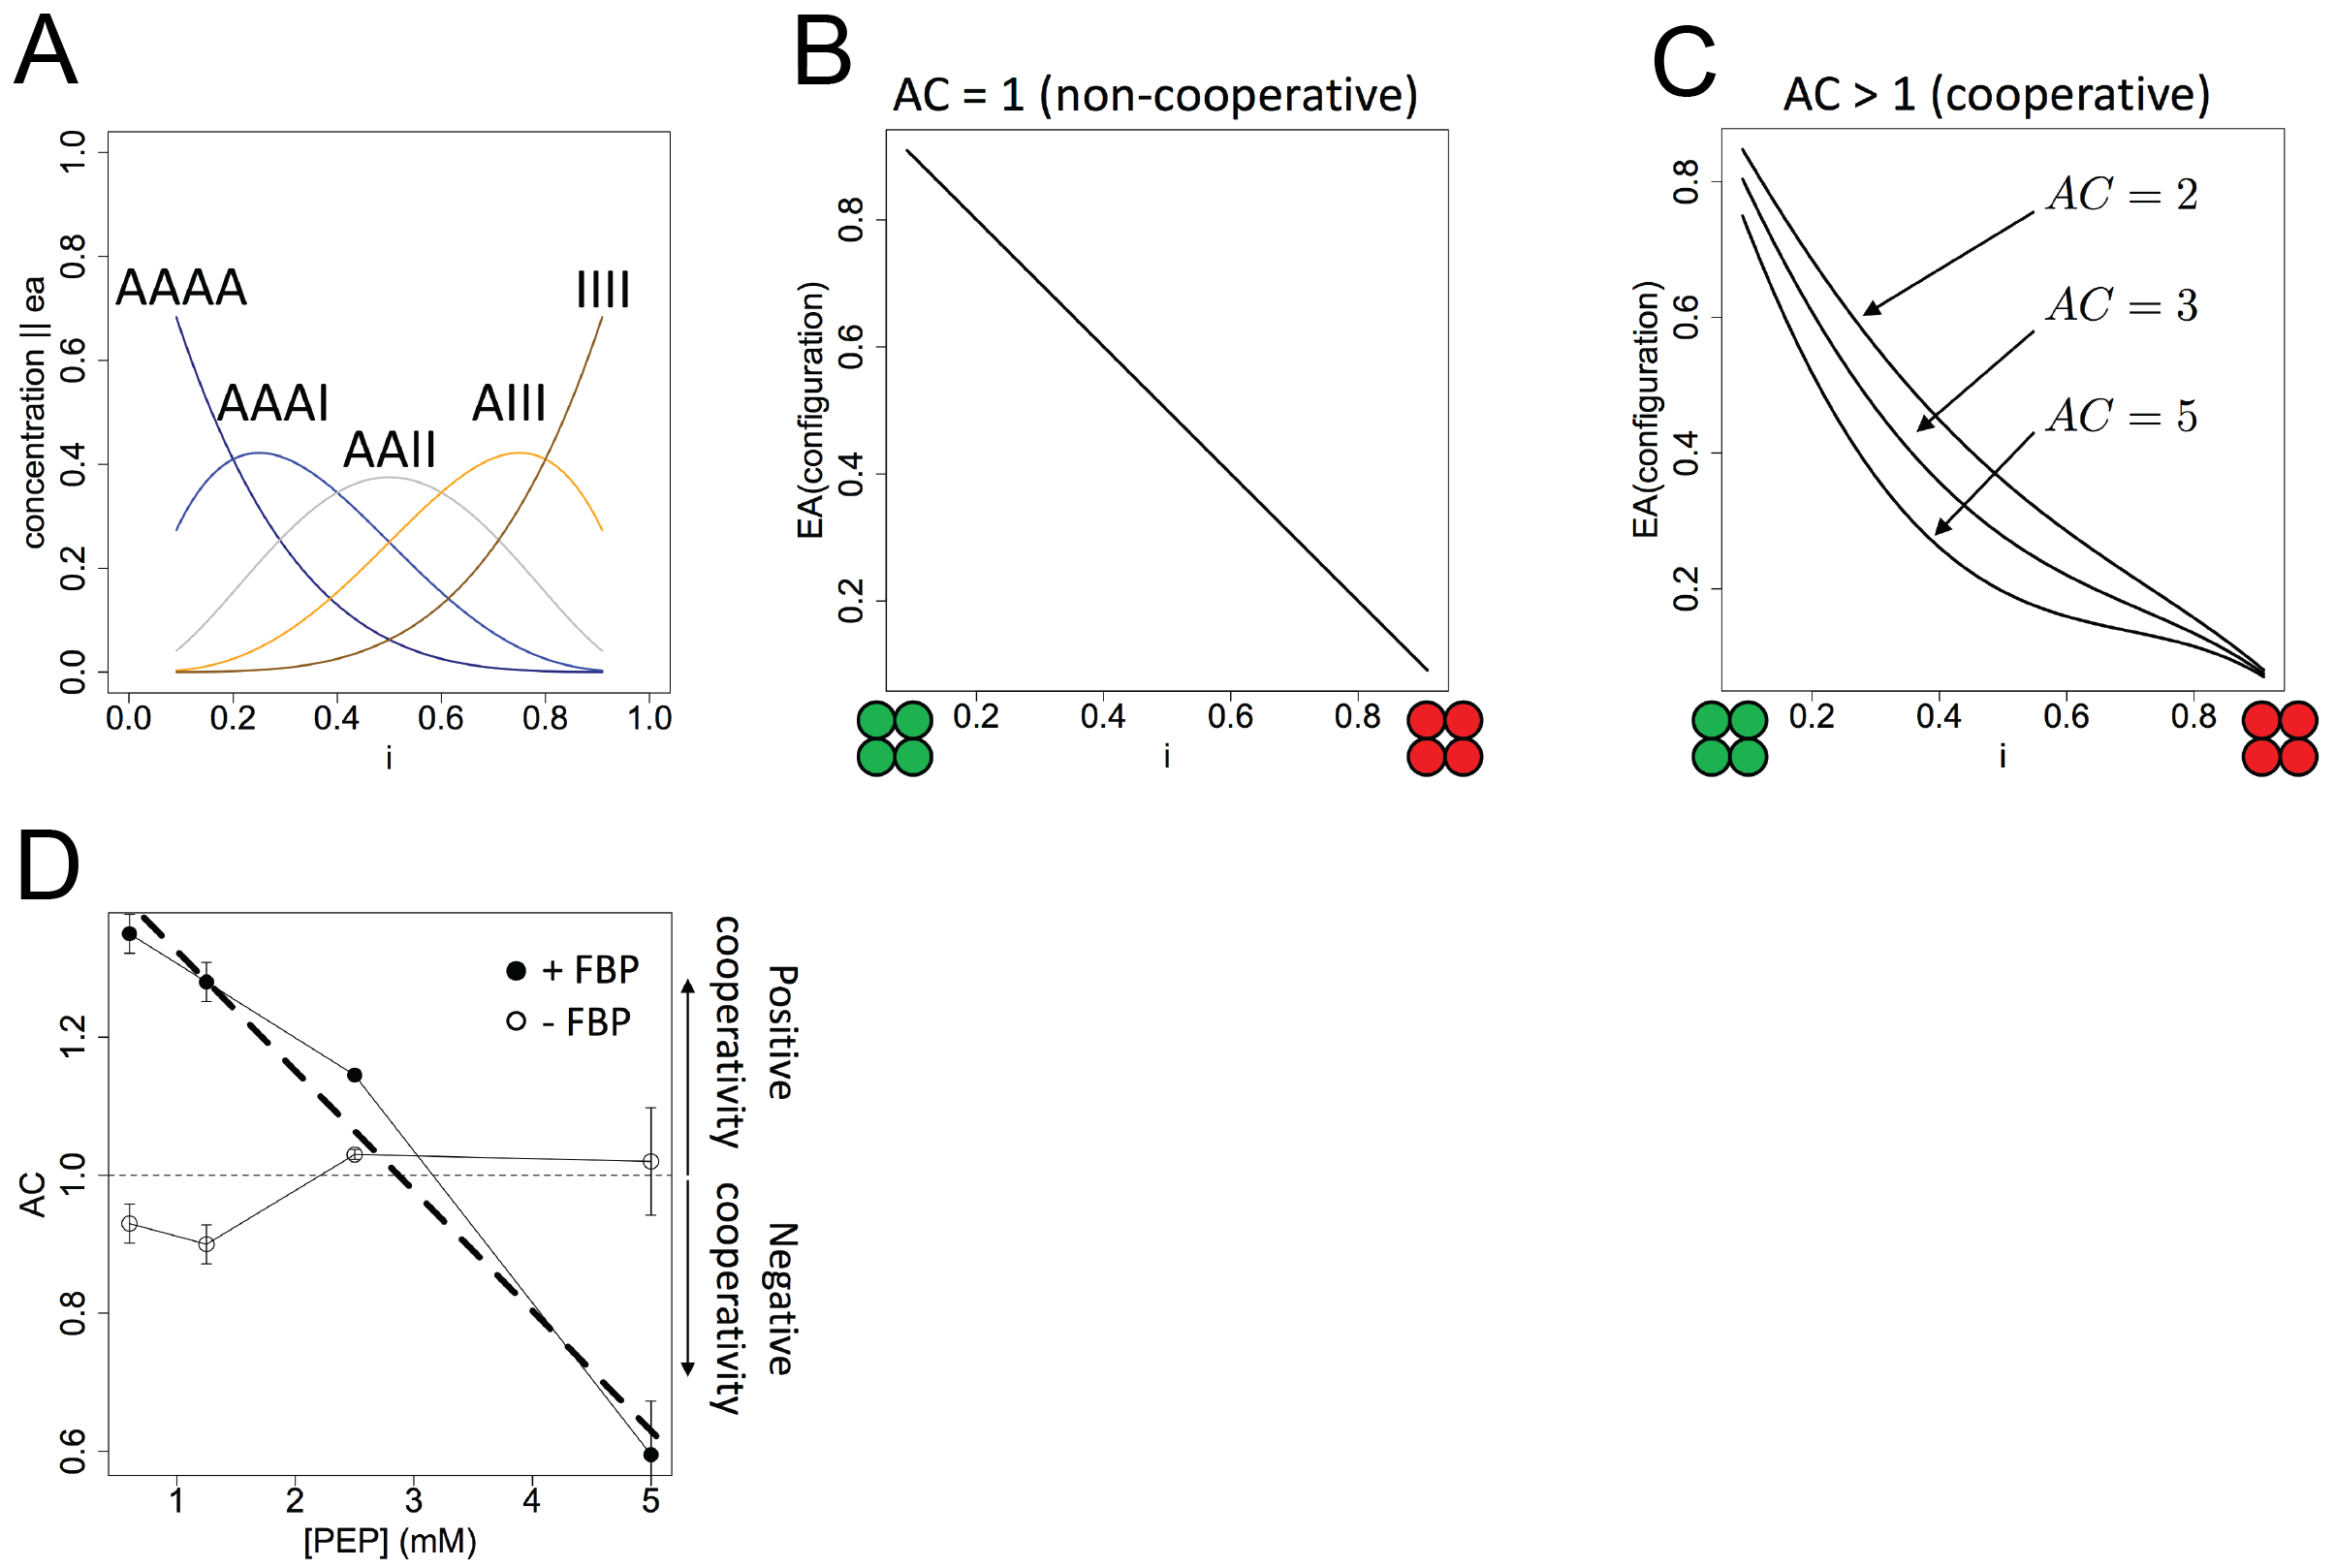
\includegraphics[scale=0.7]{ch4_fig9_mutant_doping_theory.png}
\caption[FBP binding results in inter-subunit cooperativity as defined in a numerical model.] {\textbf{FBP binding results in inter-subunit cooperativity as defined in a numerical model.} \textbf{(A)} A probability distribution for the five model hetero-oligomers AAAA, AAAI, AAII, AIIII and IIII over a range of mixtures of active and inactive protein (i). \textbf{(B)} Simulation of the decay in enzyme activity of a non-cooperative system. \textbf{(C)} Simulation in the decay in enzyme activity for a cooperative system, where increasing allosteric coefficients ($AC$) model the magnitude of inter-subunit cooperativity. \textbf{(D)} Solution for the allosteric cooperativity coefficient for WT:R72A mixtures in the absence of any added FBP (empty) and in the presence of 2 $\mu$M FBP (solid).}
\label{fig:mut_doping_theory}
\end{figure}
%
%
\clearpage

\section{FBP and amino acids combinatorially regulate PKM2 activity}
In addition to the functional effects of FBP on PKM2, demonstrated here, several amino acids compete for a common allosteric pocket \cite{Yuan:2018aa,Morgan:2013aa,Chaneton:2012aa} to regulate PKM2 enzyme activity. The regulatory effects of amino-acid binding \textit{per se} is disputed; some studies have reported allosteric effects on substrate affinity \cite{Ashizawa:1990aa,Ikeda:1998aa,Sparmann:1973aa,Chaneton:2012aa}, while others report effects on the rate of substrate turnover \cite{Morgan:2013aa,Yuan:2018aa}. Moreover, little is known about how simultaneous binding of FBP and amino acids concurrently regulate PKM2.

\subsection{Phe and Ser \textit{per se} are K-type modulators of PKM2 catalytic activity}
\label{subsec:phe_ser_fbp_activity}
To this end, we started by measuring the functional effects of an activating amino acid (L-serine; Ser) and an inhibitory amino acid (L-phenylalanine; Phe) on PKM2 enzyme catalysis \textit{per se}. Phe and Ser were chosen because their binding had been structurally resolved \cite{Chaneton:2012aa,Morgan:2013aa}, though at the time of writing a subsequent study by Yuan \textit{et al.} (2018) \cite{Yuan:2018aa} reported further structures of PKM2 in complex with Ala, Trp and His. PKM2 enzyme activity was measured in the absence and in the presence of Ser and Phe. Consistent with previously published findings, we found Phe addition to increase the Michaelis-Menten constant for the substrate $K_{M}^{PEP}$ to (7.09 $\pm$ 1.58) mM, without a detectable effect on the product turnover number [$k_{cat}$ = (324.7 $\pm$ 23.0) $s^{-1}$] (\textbf{Fig. \ref{fig:AA_activity}}). Conversely, addition of Ser resulted in a decrease in the $K_{M}^{PEP}$ to (0.22 $\pm$ 0.03) mM, without a significant change in the rate of product turnover (\textbf{Fig. \ref{fig:AA_activity}}). These results show that, in agreement with several existing studies \cite{Ashizawa:1990aa,Ikeda:1998aa,Sparmann:1973aa,Chaneton:2012aa}, Ser and Phe regulate PKM2 in a K-type manner \textit{per se} by modulating the apparent substrate affinity for PEP, without changing the apparent rate of substrate turnover.
%
%
%%% FIGURE
%
\begin{figure}[!ht]
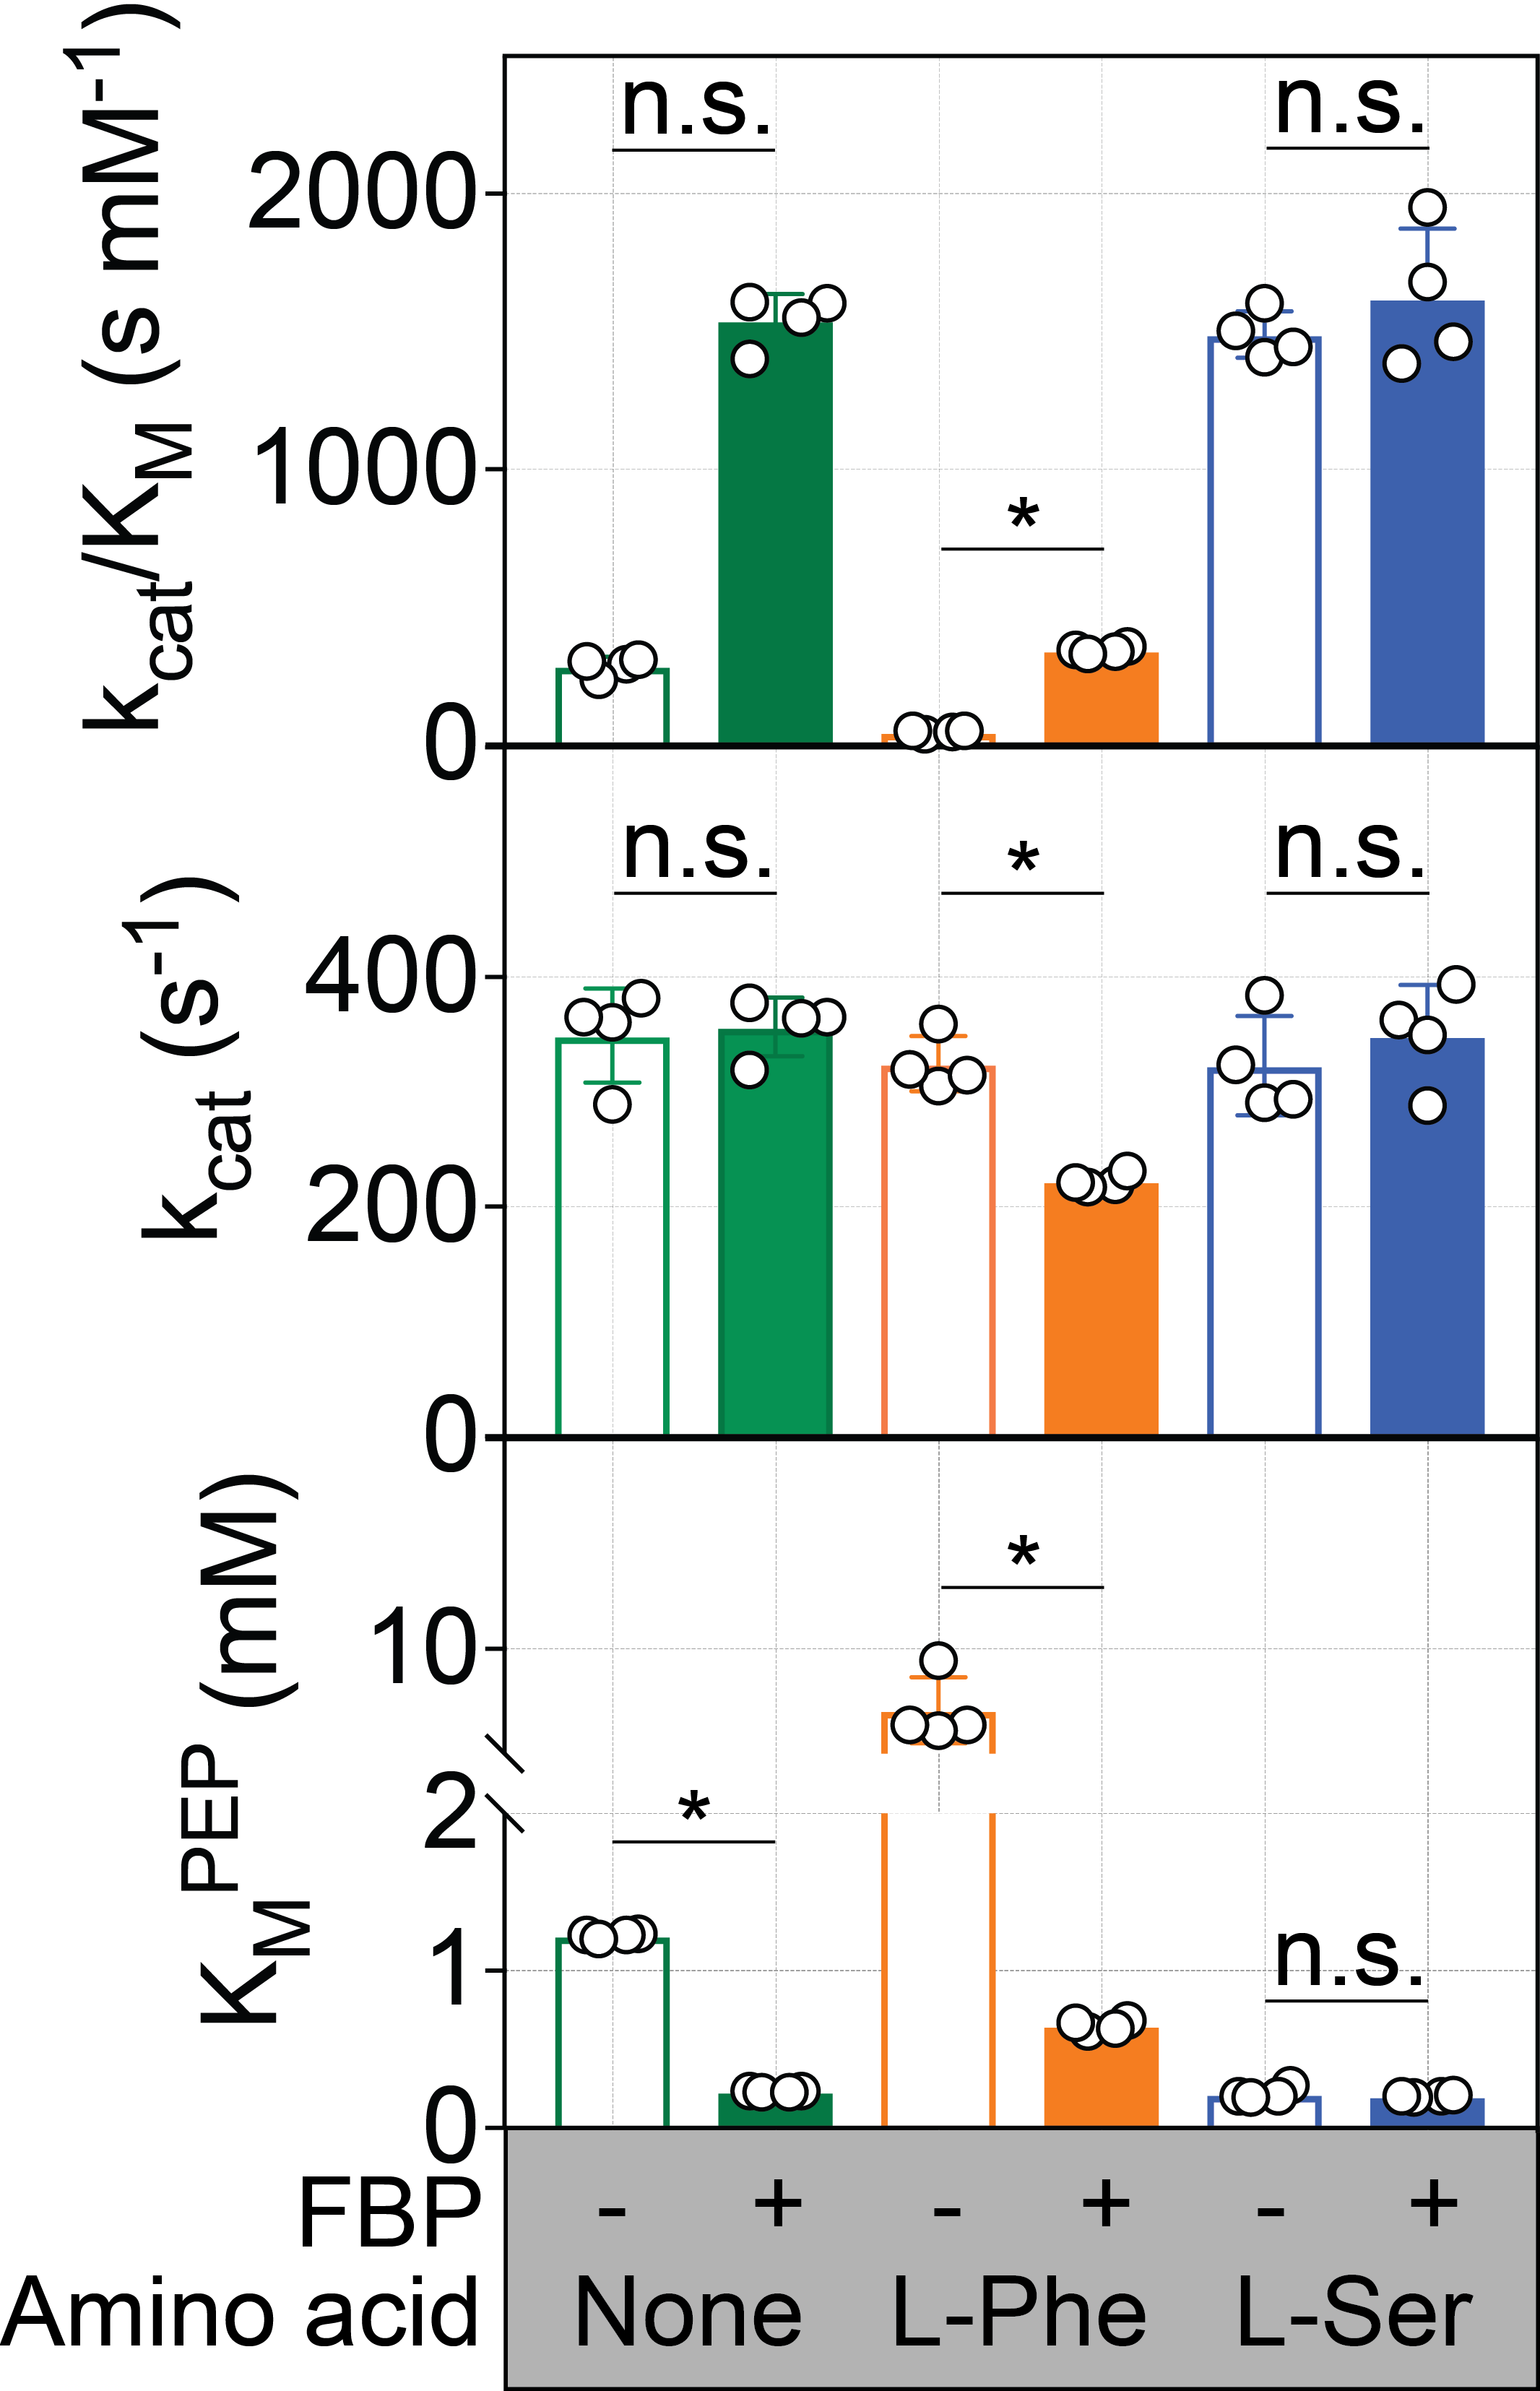
\includegraphics[scale=0.4]{ch4_fig5_AA_activity.png}
\caption[FBP and amino acids have distinct combined roles in regulating PKM2 activity.] {\textbf{FBP and amino acids have distinct combined roles in regulating PKM2 activity.} Steady-state kinetic parameters of recombinant PKM2 were measured with a spectrophotometric assay coupled to lactate dehydrogenase over a range of concentrations of the substrate phosphoenolpyruvate at 37 \textdegree C. Kinetic parameters $K_M$ and $k_{cat}$ were estimated in the absence of added ligands (empty green bars) and in the presence of 2 $\mu$M FBP (solid green), 400 $\mu$M Phe (empty orange), 400 $\mu$M  Phe and 2 $\mu$M FBP (solid orange), 200 mM Ser (empty blue) and 200 mM Ser and 2 $\mu$M FBP (solid orange). Measurements were independently repeated four times. Significance was assessed using a Wilcoxon rank-sum test. Asterisk (*) marks significant changes (p-value < 0.05). Data are shown in a tabular form in \textbf{Table \ref{tab:pkm2_activity_wildtype}}.}
\label{fig:AA_activity}
\end{figure}
%
%
\clearpage


\subsection{The mechanism of phenylalanine inhibition of PKM2 catalysis is distinct depending on FBP binding.}
\label{subsec:phe_activity_mechanism}
In order to investigate the inter-dependence between amino acid and FBP regulation, PKM2 enzyme activity was measured following addition of FBP and either Ser or Phe. Addition of Ser, subsequent to FBP did not produce detectable changes to the $K_{M}^{PEP}$ and the $k_{cat}$ (\textbf{Fig. \ref{fig:AA_activity}}), showing that FBP and Ser do not synergistically activate PKM2.

\subsubsection{In the presence of FBP, Phe reduces the substrate affinity and the maximal velocity of PKM2 catalysis}
Next, PKM2 activity was measured in the presence of FBP and Phe. We found that in the presence of FBP, Phe significantly decreased the $k_{cat}$ of PKM2 in a dose-dependent manner by 57 \% from 349.3 $s^{-1}$ at [Phe] = 0 $\mu$M, to 222.8 $s^{-1}$ at [Phe] = 400 $\mu$M. In contrast, no Phe-dependent change to the $k_{cat}$ was detected in the absence of FBP (\textbf{Fig. \ref{fig:AA_activity}}). In addition to the observed reduction in the product turnover number, Phe addition reduced the operational substrate binding affinity from 0.22 mM, in the absence of Phe and saturating FBP, to (0.65 $\pm$ 0.03) mM at [Phe] = 400 $\mu$M (\textbf{Fig. \ref{fig:AA_activity}}. Taken together, these data revealed that Phe addition, in the presence of FBP, produces a distinct inhibitory effect on PKM2 activity compared to the effects of Phe addition \textit{per se}.


\subsubsection{Phe \textit{per se} acts as a hyperbolic specific inhibitor of PKM2}
In order to assign the mechanism of Phe inhibition \textit{per se}, the dependence of the enzyme kinetic constants $K_{M}$, $k_{cat}$ and $(\frac{k_{cat}}{K_{M}})^{app}$ on the concentration of phenyalanine were analysed (as described in Methods Section \ref{subsec:methods_pkm2_phe_fbp_activity}) (\textbf{Fig. \ref{fig:phe_mechanism} A-C}). Phenylalanine was found to act as a hyperbolic specific inhibitor of PKM2 in the absence of FBP (\textbf{Fig. \ref{fig:phe_mechanism} D}). Formation of the enzyme-effector ($EX$) complex was favoured over the enzyme-substrate complex ($ES$) due to an affinity of the enzyme for Phe ($K_{X} = 0.019 \: mM$), which was approximately 14-times greater than the measured effective substrate affinity ($K_{S} = 0.250 \: mM$). However, the affinity of the substrate for the $EX$ complex was found to be very weak ($\alpha K_{S} > 20 \: mM$), thus sequestering the enzyme in the  $EX$ complex, leaving less enzyme available for the $ES$ and $ESX$ complexes, to facilitate turnover of the product. Notably, increasing concentrations of phenylalanine had little effect on the coefficient $\beta$ and so the rate of product turnover ($k_{2}$) between the $ES$ and $ESX$ complexes remained unchanged. 

\subsubsection{In the presence of FBP, Phe \textit{per se} acts as a hyperbolic mixed  inhibitor of PKM2}
The dependence of the enzyme kinetic constants $K_{M}$, $k_{cat}$ and $(\frac{k_{cat}}{K_{M}})^{app}$ on the concentration of phenyalanine was next analysed in the presence of saturating amounts of FBP (\textbf{Fig. \ref{fig:phe_mechanism} E-G}). In the presence of saturating FBP, the effective substrate binding constant to $^{FBP}E$ ($K_{S} = 0.170$  mM) was found to be approximately three-times greater than the effector binding constant ($K_{X} = 0.540$ mM), marginally favouring the formation of the $^{FBP}ES$ complex over the $^{FBP}ESX$ complex (\textbf{Fig. \ref{fig:phe_mechanism} H}). Nevertheless, Phe was found to have a significant effect on the effective substrate affinity of the $^{FBP}EX$ complex ($\alpha K_{S} = 1.130$ mM), compared to substrate binding to $^{FBP}E$, thereby acting to sequester a fraction of FBP-bound enzyme away from substrate binding. Moreover, Phe addition was found to significantly reduce the $\beta$ coefficient resulting in a reduction of the rate of product turnover from the $^{FBP}ESX$ complex ($\beta k_2 = 174.4$ $s^{-1}$), compared to the rate of product turnover from the $^{FBP}ES$ complex ($\beta k_2 = 459.0$ $s^{-1}$). Therefore, the inhibitory effect of Phe binding to $PKM2^{FBP}$ could be accounted for by a mixed mechanism of both reduced substrate binding \textit{and} reduced product turnover, and as such could be assigned as a hyperbolic mixed (predominantly specific) allosteric inhibitor of $PKM2^{FBP}$ (\textbf{Fig. \ref{fig:phe_mechanism} H}). 
%
\\\\
%
Together, these data revealed that FBP mechanistically alters the mode of PKM2 inhibition by phenylalanine from a hyperbolic specific inhibitor, to a mixed hyperbolic inhibitor. When FBP is absent, Phe acts exclusively as a K-type inhibitor whereas, in the presence of saturating concentrations of FBP, Phe addition acts on both the $K_{M}^{PEP}$ and the $k_{cat}$, as a mixed V- and K-type inhibitor.
%
%
%%% FIGURE
%
\begin{figure}[!ht]
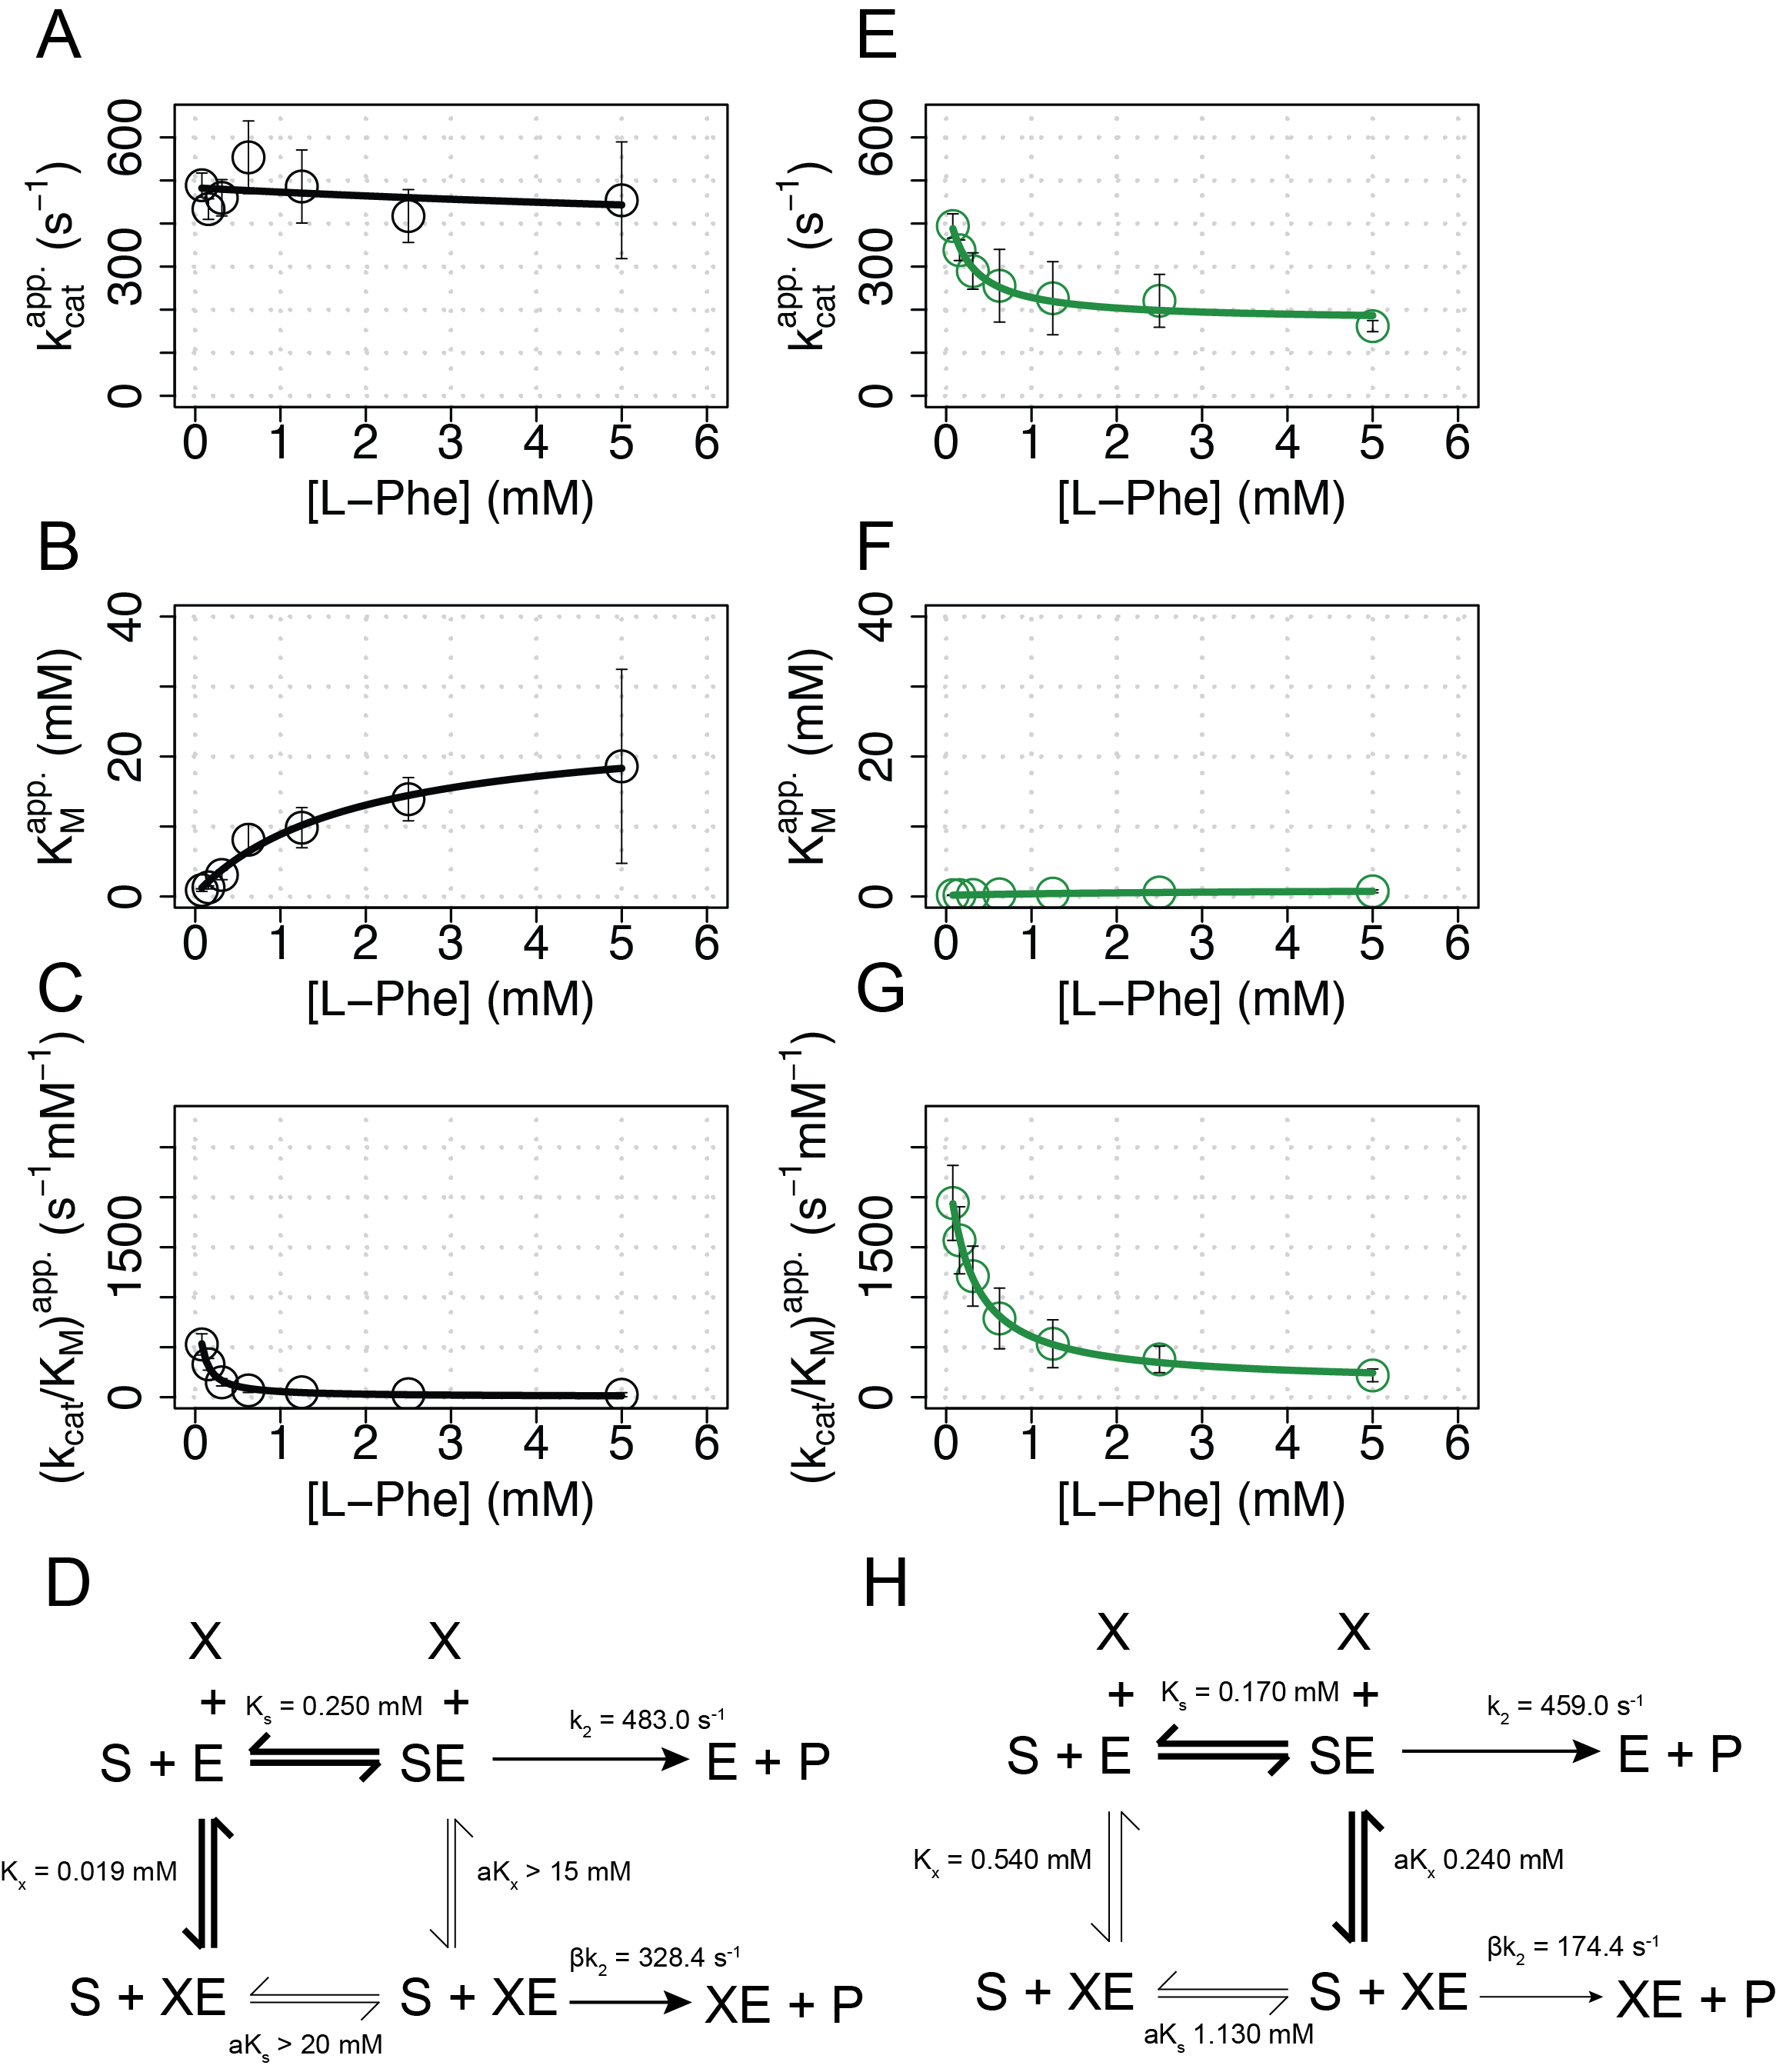
\includegraphics[scale=0.7]{ch4_fig6_phe_fbp_activity.png}
\caption[Phenylalanine inhibition follows one of two distinct mechanisms, depending on the presence of FBP.] {\textbf{Phenylalanine inhibition follows one of two distinct mechanisms, depending on the presence of FBP.} Recombinant PKM2 activity was measured at varying concentrations of PEP and a constant concentrations of 5 mM ADP and 5 nM PKM2, at 37 \textdegree C. Initial velocities were performed in the presence of a range of Phe concentrations between 0.08 mM and 5 mM. Rate curves were fitted to Michaelis-Menten kinetic models, from which the parameters $k_{cat}$, $K_{M}^{PEP}$ and $\frac{k_{cat}}{K_{M}^{PEP}}$ were computed for Phe inhibition of $PKM2^{apo \ast}$ (black; \textbf{A}, \textbf{B} and \textbf{C}). \textbf{(D)} The dependence of the three steady-state kinetic parameters $k_{cat}$, $K_{M}^{PEP}$ and $\frac{k_{cat}}{K_{M}^{PEP}}$ were fit to the steady-state modifier-rate equations defined in the text. \textbf{(E-H)} An analysis of phenylalanine inhibition was repeated as in (A-D), in the presence of 2 $\mu$M FBP (saturating amounts). }
\label{fig:phe_mechanism}
\end{figure}
%
%
%
%
%TABLE
\begin{table}[!ht]
\centering
\caption[Steady-state Michaelis-Menten kinetic parameters for $PKM2^{apo \ast}$, and following the addition of FBP, Phe and Ser.]{\textbf{Steady-state Michaelis-Menten kinetic parameters for $PKM2^{apo \ast}$, and following the addition of FBP, Phe and Ser.}}
\begin{tabular}{llll}
\hline
Ligand & $K_{M}^{PEP}$ (mM) & $k_{cat}$ ($s^{-1}$) & $\frac{k_{cat}}{K_{M}^{PEP}}$ ($s^{-1} \cdot mM^{-1}$) \\ \hline
Apo$\ast$ & 1.22 $\pm$ 0.02 & 349.3 $\pm$ 40.9 & 285.6 $\pm$ 34.1 \\
Phe & 7.08 $\pm$ 1.58 & 324.7 $\pm$ 23.9 & 46.8 $\pm$ 6.0 \\
Ser & 0.22 $\pm$ 0.04 & 323.1 $\pm$ 43.2 & 1489.8 $\pm$ 84.7 \\
FBP & 0.23 $\pm$ 0.04 & 356.7 $\pm$ 25.7 & 1540.4 $\pm$ 96.9 \\
FBP and Phe & 0.65 $\pm$ 0.03 & 222.3 $\pm$ 6.3 & 342.1 $\pm$ 11.1 \\
FBP and Ser & 0.20 $\pm$ 0.04 & 348.7 $\pm$ 44.3 & 1620.0 $\pm$ 253.6 \\ \hline
\end{tabular}
\label{tab:pkm2_activity_wildtype}
\end{table}

\clearpage


\subsection{Ligand-induced changes in affinity cannot explain the changed phenylalanine-inhibition of PKM2 by FBP}
Results in Sections \ref{subsec:phe_ser_fbp_activity} and \ref{subsec:phe_activity_mechanism} revealed that FBP addition changes the inhibition kinetics of Phe. It was unclear whether this was a result of a combinatorial effect of both ligands on the bind affinity of the other, or whether the result reflected a \textit{bona fide} functional cross-talk between the two ligands. Indeed, the effective Phe binding constant to $PKM2^{apo \ast}$ [$K_{X}^{apo \ast}$ = (0.019 $\pm$ 0.077)  mM] was found to be significantly different compared to that of Phe binding to $PKM2^{FBP}$ [$K_{X}^{FBP}$ = (0.540 $\pm$ 0.06)  mM] (\textbf{Fig. \ref{fig:phe_mechanism} D} and \textbf{H}). Nevertheless, since a simplified single-substrate-single-enzyme mechanism was assumed, it was unclear whether the changed ($K_{X}$) reflected a changed binding affinity or whether a more complex interaction between PKM2, phosphoenolpyruvate and adenosine diphosphate (the second substrate not considered in the above mechanism) was at play. To this end, the mutual effects of FBP and amino acids on binding to PKM2 was investigated. 
%
%
\\\\
%
%
We first estimated the apparent affinities of each ligand in the presence of saturating amounts of the other. In the presence of saturating concentrations of either Phe or Ser, the $K_D^{FBP}$ decreased, however this was found not to be statistically significant (p = 0.150 and p = 0.054, respectively) (\textbf{Fig. \ref{fig:AA_binding} A}).
%
\\\\
%
Next, the binding of Phe and Ser to PKM2 was measured, in the absence and in the presence of FBP, using MST. Phe and Ser addition to PKM2 produced dose-dependent changes to the thermophoresis of labelled PKM2. The estimated binding affinites of Phe [(191.0 $\pm$ 86.2) $\mu$M) and Ser [(507.5 $\pm$ 218.8) $\mu$M) (\textbf{Fig. \ref{fig:AA_binding} B}), were unaffected by the addition of saturating amounts of FBP (\textbf{Fig. \ref{fig:AA_binding} C}).
%
%
\\\\
%
%
Taken together, these measurements suggested that alteration in the binding affinity of one ligand by the presence of the other cannot account for the distinct FBP-dependent modes of PKM2 inhibition by Phe. Rather, the altered mechanism of Phe inhibition upon FBP binding may reflect a mechanistic dependence between the two allosteric regulators.
%
%
%%% FIGURE
%
\begin{figure}[!ht]
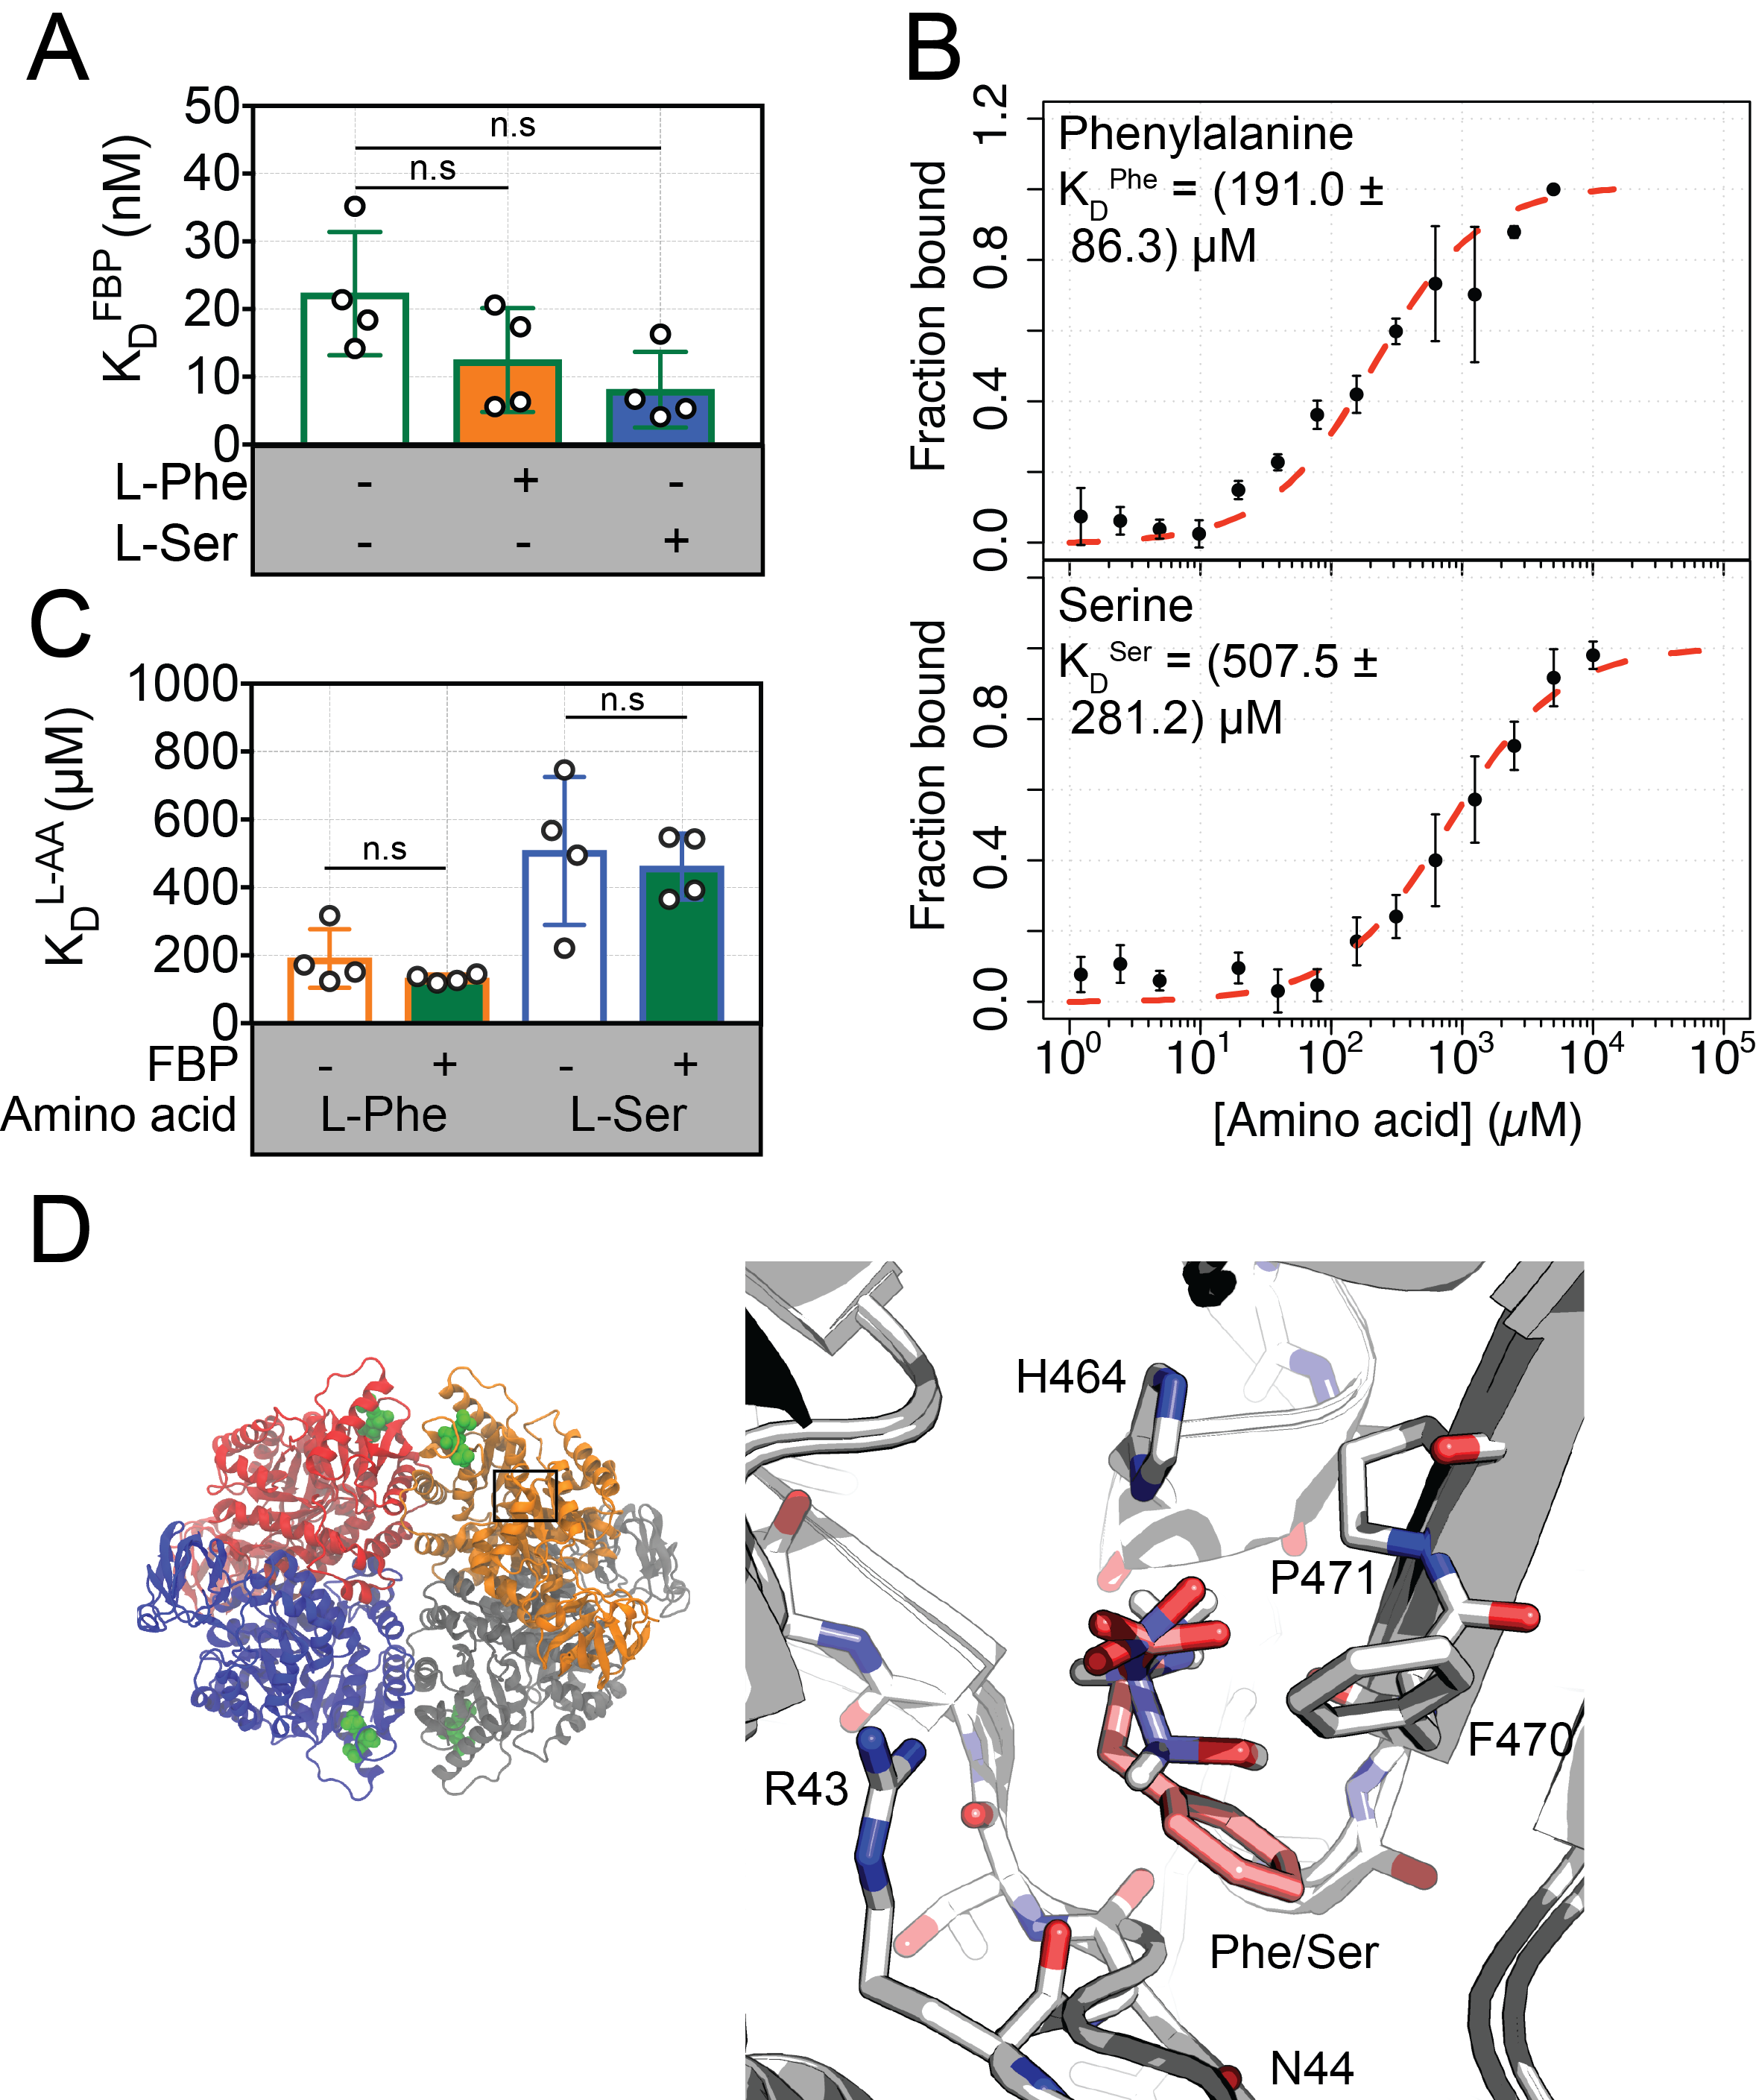
\includegraphics[scale=0.7]{ch4_fig7_FBP_AA_binding.png}
\caption[Amino acids and FBP do not reciprocally affect binding.] {\textbf{Amino acids and FBP do not reciprocally affect binding.} \textbf{(A)} FBP binding to PKM2 was measured using fluorescence emission spectroscopy (as described previously) in the absence of amino acids (green) and in the presence of 400 $\mu$M Phe (orange) and 200 mM Ser. \textbf{(B)} MST measurements of fluorescein-labelled PKM2 were performed to monitor serine (Ser) and phenylalanine (Phe) binding to PKM2. Labelled PKM2, at a constant concentration of 30 nM, was titrated with either Phe or Ser, and the thermophoretic properties of the resulting protein-ligand interaction was measured. The mean and standard deviations of four separate titrations are shown. \textbf{(C)} MST experiments were repeated for Phe (orange) and Ser (blue) in the presence of 2 $\mu$M FBP. \textbf{(D)} The overlapping modes of Phe and Ser binding to PKM2 are superimposed from two crystal structures \cite{Chaneton:2012aa,Morgan:2013aa}.}
\label{fig:AA_binding}
\end{figure}
\clearpage




\section{Simultaneous regulation of PKM2 by multiple ligands is relevant for enzyme regulation in cells} \label{Simultaneous regulation of PKM2 by multiple ligands is relevant for enzyme regulation in cells}
Results presented in this chapter demonstrate that FBP binds tightly to PKM2 with a high affinity, and that Phe attenuates FBP-induced activation by stabilising a distinct kinetic state with a reduced maximal velocity. The fraction of PKM2 bound to allosteric ligands in cells, and hence the ability of these ligands to exert their respective regulatory effects, is determined by their intracellular concentrations and their binding affinities. To investigate whether FBP and amino acids are likely to concurrently bind to PKM2 and whether this is relevant for PKM2 regulation, we sought to quantify the fractional saturation of PKM2 bound to FBP, Ser and Phe, in proliferating cancer cells. The cellular fraction of PKM2 bound to allosteric ligands is given by:
%
%
\begin{equation}
[PL] = \frac{(K_{D} + [P_{ic}] + [X_{ic}]) - \sqrt{(K_{D} + [P_{ic}] + [X_{ic}])^{2} - 4(P_{ic}[X_{ic}])}}{2}
\end{equation}
%
%
\begin{equation}
s = \frac{[PL]}{[P_{ic}]}
\label{equ:saturation}
\end{equation}
%
%
where $[P_{ic}]$ and $[X_{ic}]$ are the intracellular protein and metabolite concentrations, respectively. 

\subsection{Intracellular FBP binding to PKM2 is constitutive whereas Phe and Ser bind reversibly}
\label{subsec:ic_concentrations}

\subsubsection{The intracellular concentration of FBP is in excess of its binding affinity to PKM2}
To this end, the range of intracellular concentrations of FBP, Ser and Phe in three human cancer cells lines of different tissue origin (HCT116, LN229 and SN12C), cultured in the presence of physiological (human blood serum) concentrations of glucose ($Gluc^{+}$). $[FBP]_{ic}$ varied between between 240-360 $\mu$M across the three cell lines (\textbf{Fig. \ref{fig:ligand_IC} A}). This concentration range of FBP, under physiological glucose culture conditions, was in excess of the $K_{D}^{FBP}$ between 11919- and 17755-fold. The fraction of cellular PKM2 bound to FBP, calculated using \textbf{Equ. \ref{equ:saturation}}, found a fractional saturation of 0.99, which remained unchanged even in cells cultured in the absence of glucose ($Gluc^{-}$) (\textbf{Fig. \ref{fig:ligand_IC} B}), despite a marked reduction in the $[FBP]_{ic}$ to between 20-70 $\mu$M across the three cell lines.


\subsubsection{The intracellular concentrations of Ser and Phe constitute a dynamic range around their respective affinities for PKM2}
Next, cells were supplemented with either 100 $\mu$M Ser and 500 $\mu$M Phe ($S^{100}F^{500}$) or 500 $\mu$M Ser and 100 $\mu$M Phe $S^{100}F^{500}$). Under physiological media concentrations, the intracellular concentrations varied between 200-320 $\mu$M for Phe and 2000-4000 $\mu$M for Ser, across the three cell lines (\textbf{Fig. \ref{fig:ligand_IC} C}). The measured $[Phe]_{ic}$ and $[Ser]_{ic}$ were close to the apparent binding affinities for PKM2 [$K_{D}^{Phe}$ = (191.0 $\pm$ 86.3) $\mu$M and $K_{D}^{Ser}$ = (507.5 $\pm$ 218.2) $\mu$M]. The associated fractional saturation of PKM2 with Phe was between 0.53-0.75, and between 0.81 and 0.92 with Ser. The range of predicted fractional saturations in the complete absence of amino acids ($aa^{-}$) or 5x physiological concentrations was 0.05 and 0.18 for Phe and Ser, respectively, in culture conditions devoid of amino acids ($aa^{-}$). The fractional saturation of both Phe and Ser was found to increase to 0.90 and 0.98, respectively, in conditions of $S^{100}F^{500}$ and $S^{500}F^{100}$ (\textbf{Fig. \ref{fig:ligand_IC} D}). 
%
%
\\\\
%
%
Estimations for the fraction of PKM2 bound to Ser and Phe did not take into account the fact that these two ligands compete for binding. Moreover, the calculation assumed that binding was unaffected by other amino acids, which have been shown to bind competitively at the same allosteric pocket \cite{Yuan:2018aa}. As such, the predicted fractional saturation of Phe and Ser is likely to be an under-estimation of the true cellular value. Conversely, FBP binding was predicted to be constitutively saturated, evidenced by a predicted binding saturation approaching 1 in all conditions (\textbf{Fig. \ref{fig:ligand_IC} D}).
%
%
%
%%% FIGURE
%
\begin{figure}[!ht]
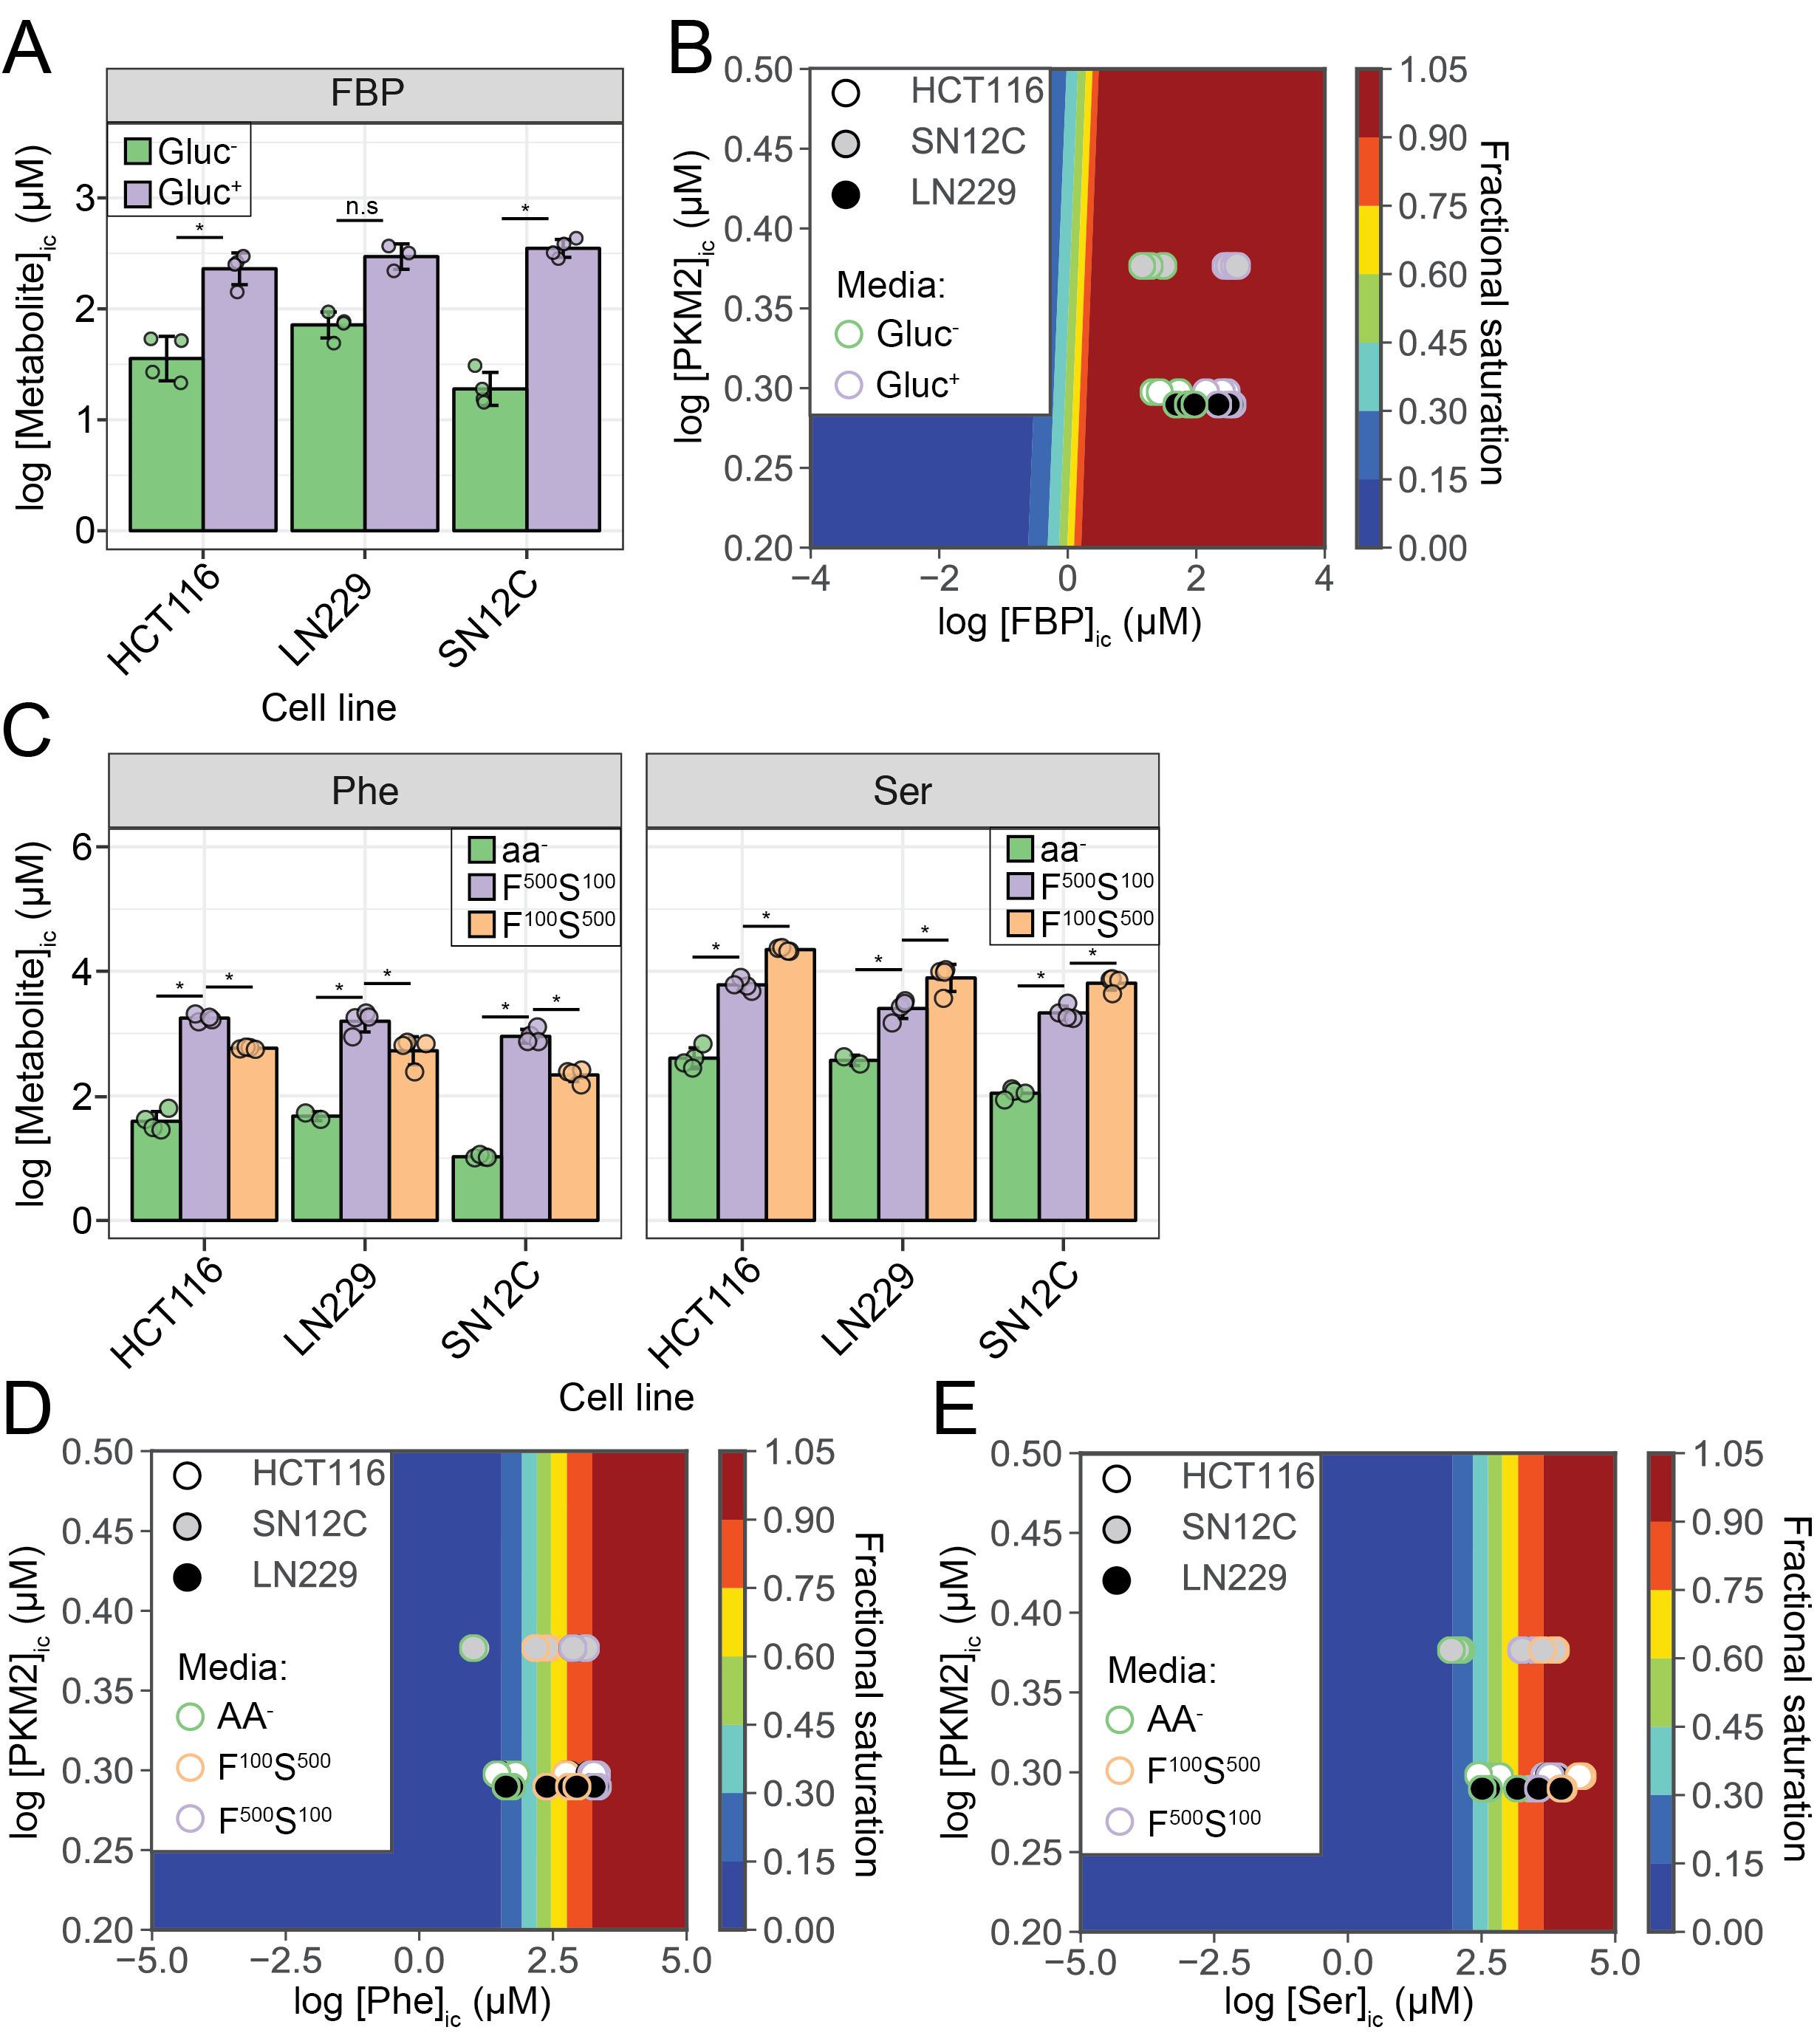
\includegraphics[scale=0.6]{ch4_fig10_cellular_lig_conc.png}
\caption[Cellular concentrations of PKM2 allosteric effectors reveal a physiological role for multi-ligand regulation.] {\textbf{Cellular concentrations of PKM2 allosteric effectors reveal a physiological role for multi-ligand regulation.} \textbf{(A)} Intracellular concentrations of FBP were measured using liquid-chromatography mass spectrometry (LC-MS) from HCT116, LN229 and SN12C cells cultured in fully-fed conditions (RPMI containing 11 mM glucose; green bars) and glucose-deprived conditions (RPMI containing 0 mM glucose; purple bars) for 1 hour. \textbf{(B)} A phase diagram for intracellular FBP binding to PKM2 was computed over a range of [FBP] and [PKM2] values. Saturation of ligand-protein binding is represented by a colour scale; a fractional saturation approaching 0 indicating conditions under which PKM2 is fully \textit{apo$\ast$} with respect to its interaction with FBP, and a fractional saturation equal to 1 indicates that each FBP binding site on the cellular pool of PKM2 is occupied. The predicted fractional saturation for each of the three cell lines (four technical replicates) are shown in the phase diagram. The intracellular concentration of PKM2 was measured for each cell line using a targeted proteomics approach (see Methods Section \ref{subsec:methods_pkm2_proteomics}). \textbf{(C)} Intraceullar concentrations of Phe and Ser were measured in media devoid of amino acids ($aa^{-}$), containing 500 $\mu$M Phe and 100 $\mu$M Ser ($F^{500}S^{100}$) or 100 $\mu$M Phe and 500 $\mu$M Ser ($F^{500}S^{100}$). Phase diagrams were computed for phenylalanine \textbf{(D)} and serine \textbf{(E)}, as for FBP above.}
\label{fig:ligand_IC}
\end{figure}
%
%
\clearpage


\subsection{The addition of exogenous FBP does not change PKM2 activity in HCT116 cell lysates}
\label{subsec:cell_lysate_act_fbp}
Under conditions where FBP binding is constitutive, the intracellular activity of PKM2 would be predicted to be unresponsive to the addition of further amounts of exogenous FBP. To test this hypothesis, we assayed HCT116 cell lysates for PKM2 activity, following culture in glucose-fed and glucose-depleted media. Cells were gently lysed in hypotonic lysis buffer, in an attempt to maintain the intracellular FBP-PKM2 stoichiometry. It was observed that, while addition of 100 $\mu$M FBP to recombinant PKM2 had the effect of decreasing the $K_{M}^{PEP}$ by 7-fold, very little change to PKM2 activity was apparent in HCT116 lysates upon addition of up to 1 mM exogenous FBP (\textbf{Fig. \ref{fig:lysate_activity} A}). 

\subsubsection{Phe addition reduces the maximal velocity of PKM2 activity in cell lysates}
Addition of physiological concentrations of exogenous Phe to HCT116 cell lysates resulted in an apparent inhibition of PKM2 activity, and a dose-dependent reduction in the $\frac{k_{cat}}{K_{M}^{PEP}}$ (\textbf{Fig. \ref{fig:lysate_activity} B}). It was observed that a Phe dose-depedent reduction in the maximal velocity was the main kinetic determinant in the inhibition of the $\frac{k_{cat}}{K_{M}^{PEP}}$ of PKM2. No detectable change to the ${K_{M}^{PEP}}$, however, was apparent upon addition of Phe to HCT116 lysates, similar to the observed mechanism of Phe inhibition of recombinant $PKM2^{FBP}$. Furthermore, the addition of exogenous molar concentrations of Ser out-competed the inhibitory effect of Phe, restoring the maximal velocity to 'FBP-bound' levels (\textbf{Fig. \ref{fig:lysate_activity} C}). 

\subsubsection{Binding of PKM2 to PEP in cells is predicted to be sub-saturating}
Intracellular concentrations of the catalytic substrate phosphoenolpyruvate (PEP) were measured in the low micro-molar range between (9.6 $\pm$ 3.5) $\mu$M and (2.3 $\pm$ 1.3) $\mu$M under glucose-fed and glucose-deprived conditions, respectively (\textbf{Fig. \ref{fig:pep_conc} A}). The estimated ${K_{A}^{PEP}}$ was therefore between approximately 24-fold and 100-fold in excess of $[PEP]_{ic}$, suggesting that a very low fraction of the protein was bound to its substrate in cells ($s_{PEP} < 0.04$) (\textbf{Fig. \ref{fig:pep_conc} B}). Conditions where the substrate is limiting give further credence to the relevance of Phe and Ser competitively modulating the rate of product turnover, in the context of constitutive FBP binding. Nevertheless, possible channelling of the substrate and/or differential PEP sequestration in different cellular compartments, could not be discounted.
%
%
%
%%% FIGURE
%
\begin{figure}[!ht]
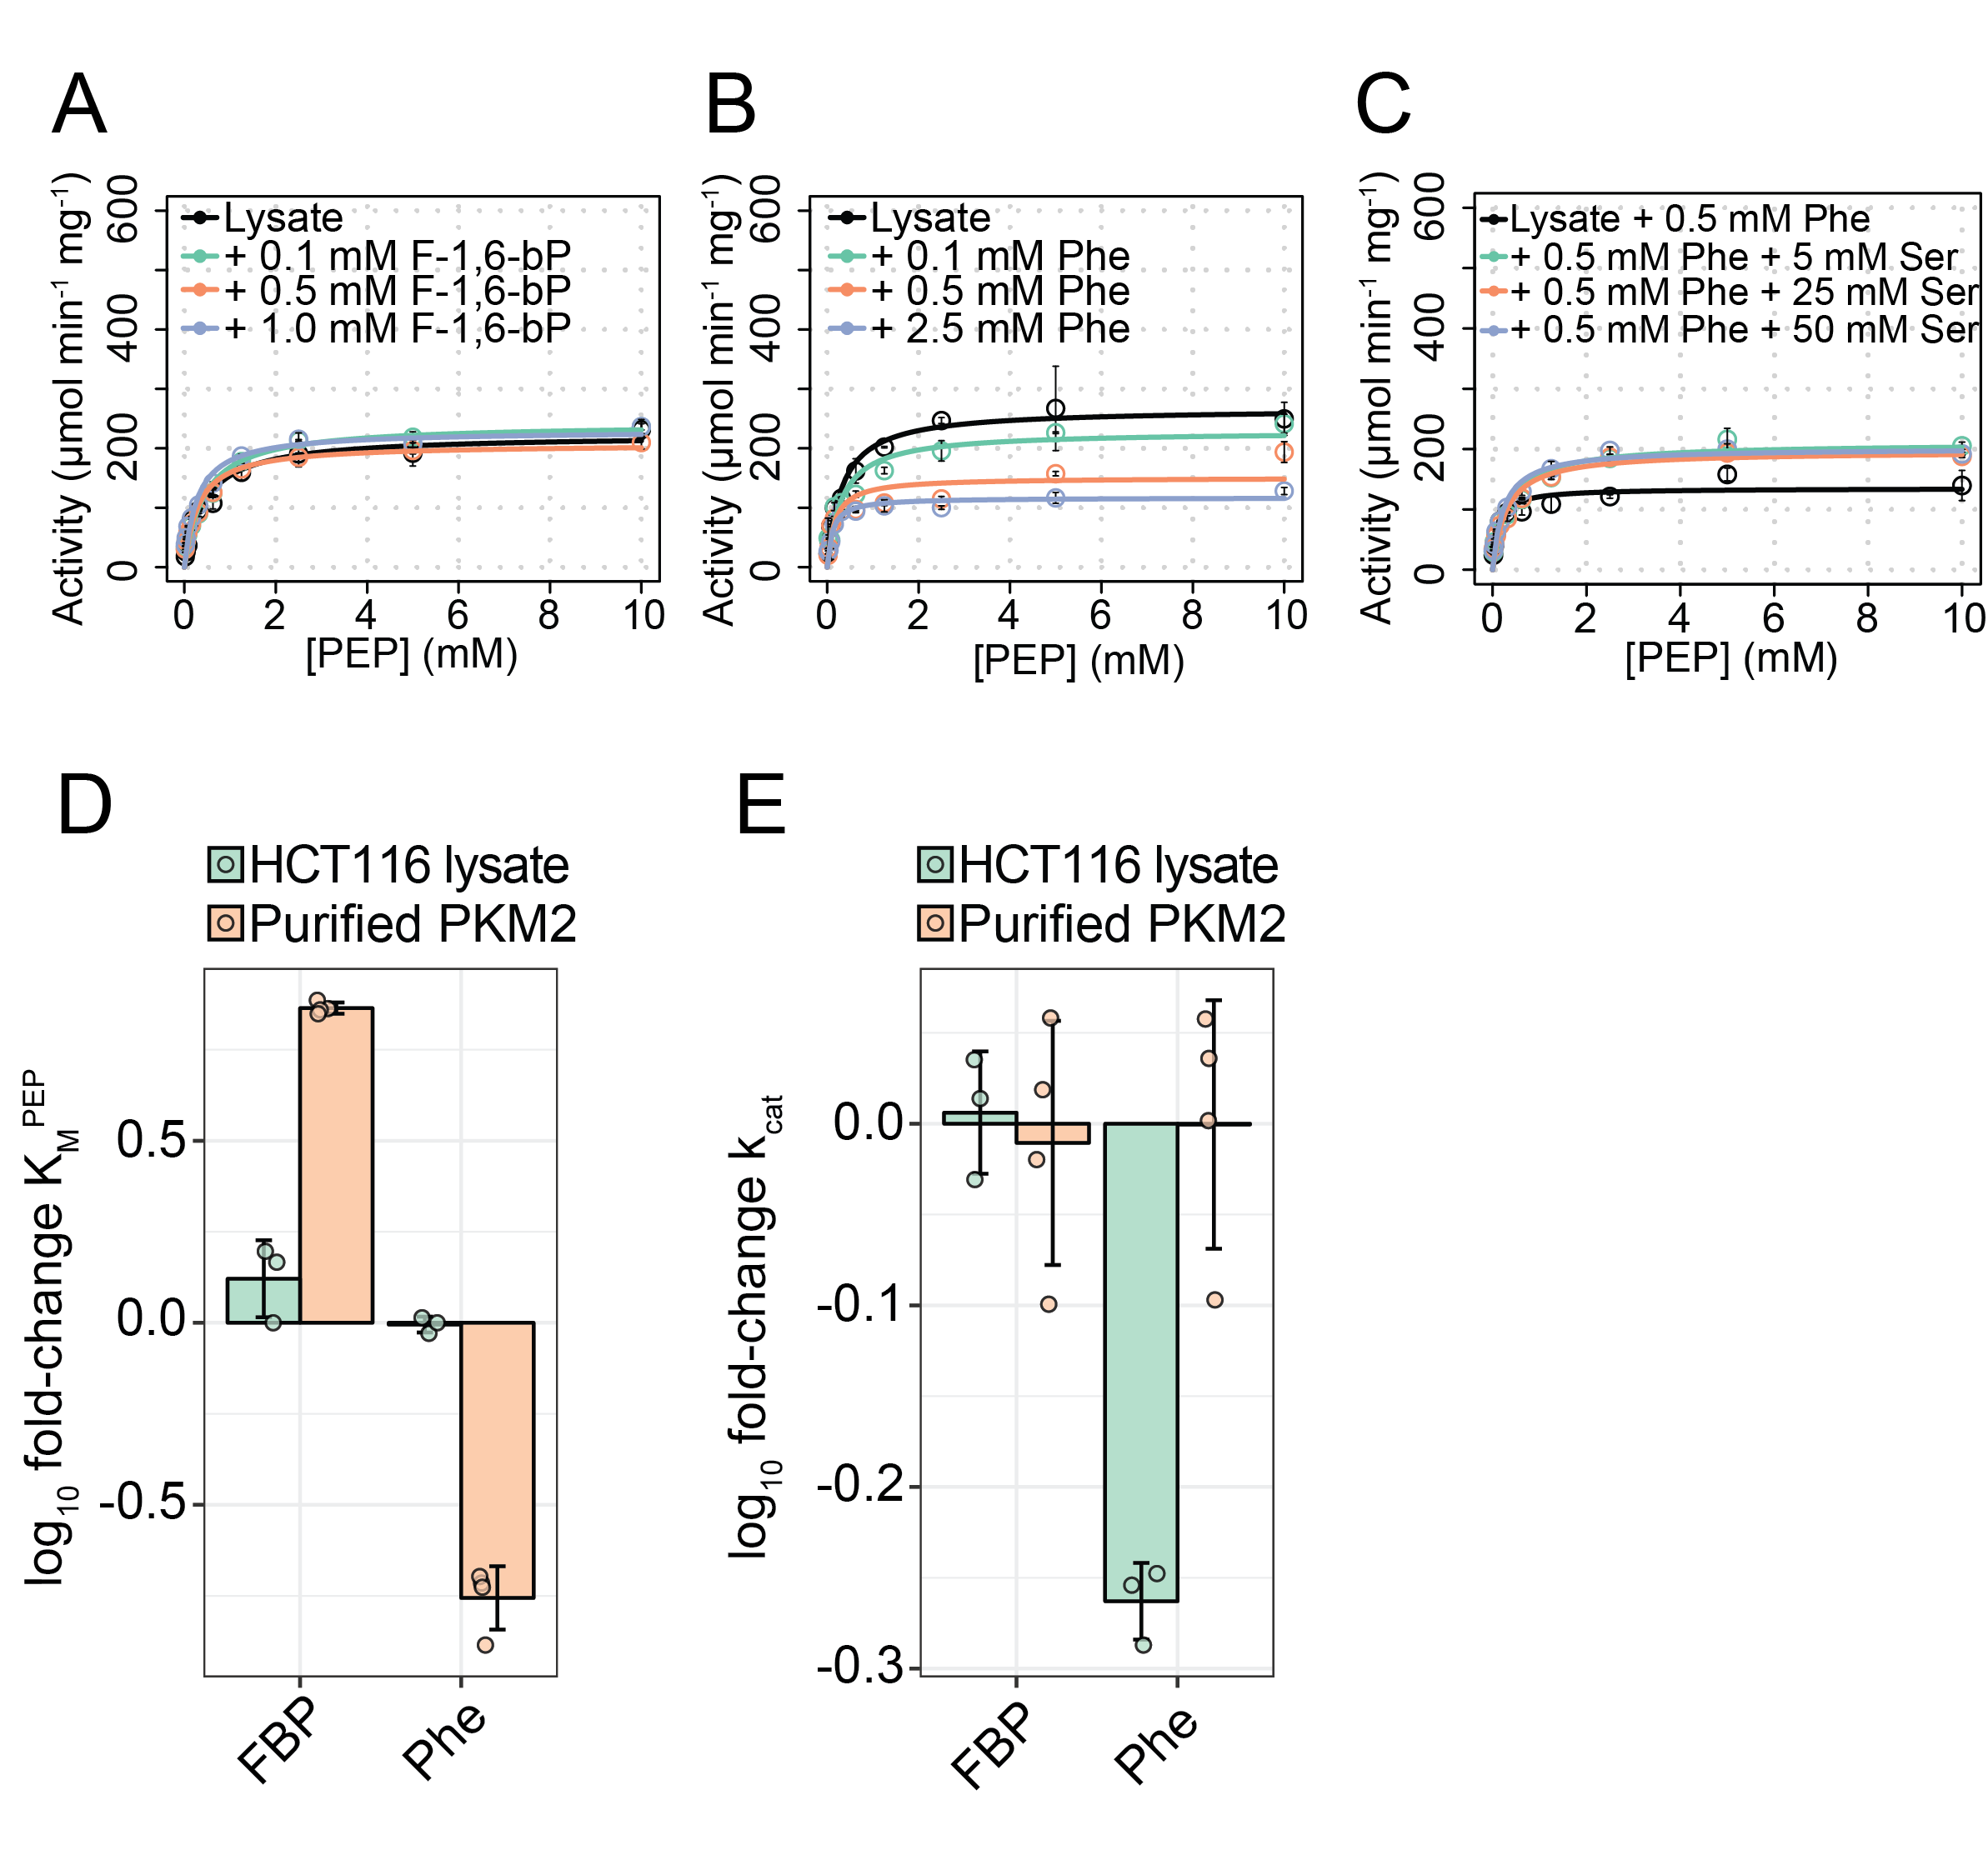
\includegraphics[scale=0.7]{ch4_fig11_lysate_activity.png}
\caption[PKM2 activity from HCT116 lysates is not further activated by addition of exogenous FBP.] {\textbf{PKM2 activity from HCT116 lysates is not further activated by addition of exogenous FBP.} \textbf{(A)} PKM2 activity in HCT116 cells cultured under glucose-fed conditions was assayed, in the presence of increasing concentrations of exogenously added FBP. Initial velocities were measured over a range of PEP concentrations. \textbf{(B)} Activity measurements were repeated in presence of increasing concentrations of exogenous phenylalanine and \textbf{(C)} serine. The fold-change in the Michaelis-Menten constants \textbf{(D)} $K_{M}^{PEP}$ and $k_{cat}$ measured from PKM2 activity of recombinant PKM2 (orange) and PKM2 activity in HCT116 cell lysates (teal). The fold-change is plotted between the 'apo$\ast$' condition and upon addition of either 2 $\mu$M FBP or 400 $\mu$M Phe.}
\label{fig:lysate_activity}
\end{figure}
%
%
%
%
%
%%% FIGURE
%
\begin{figure}[!ht]
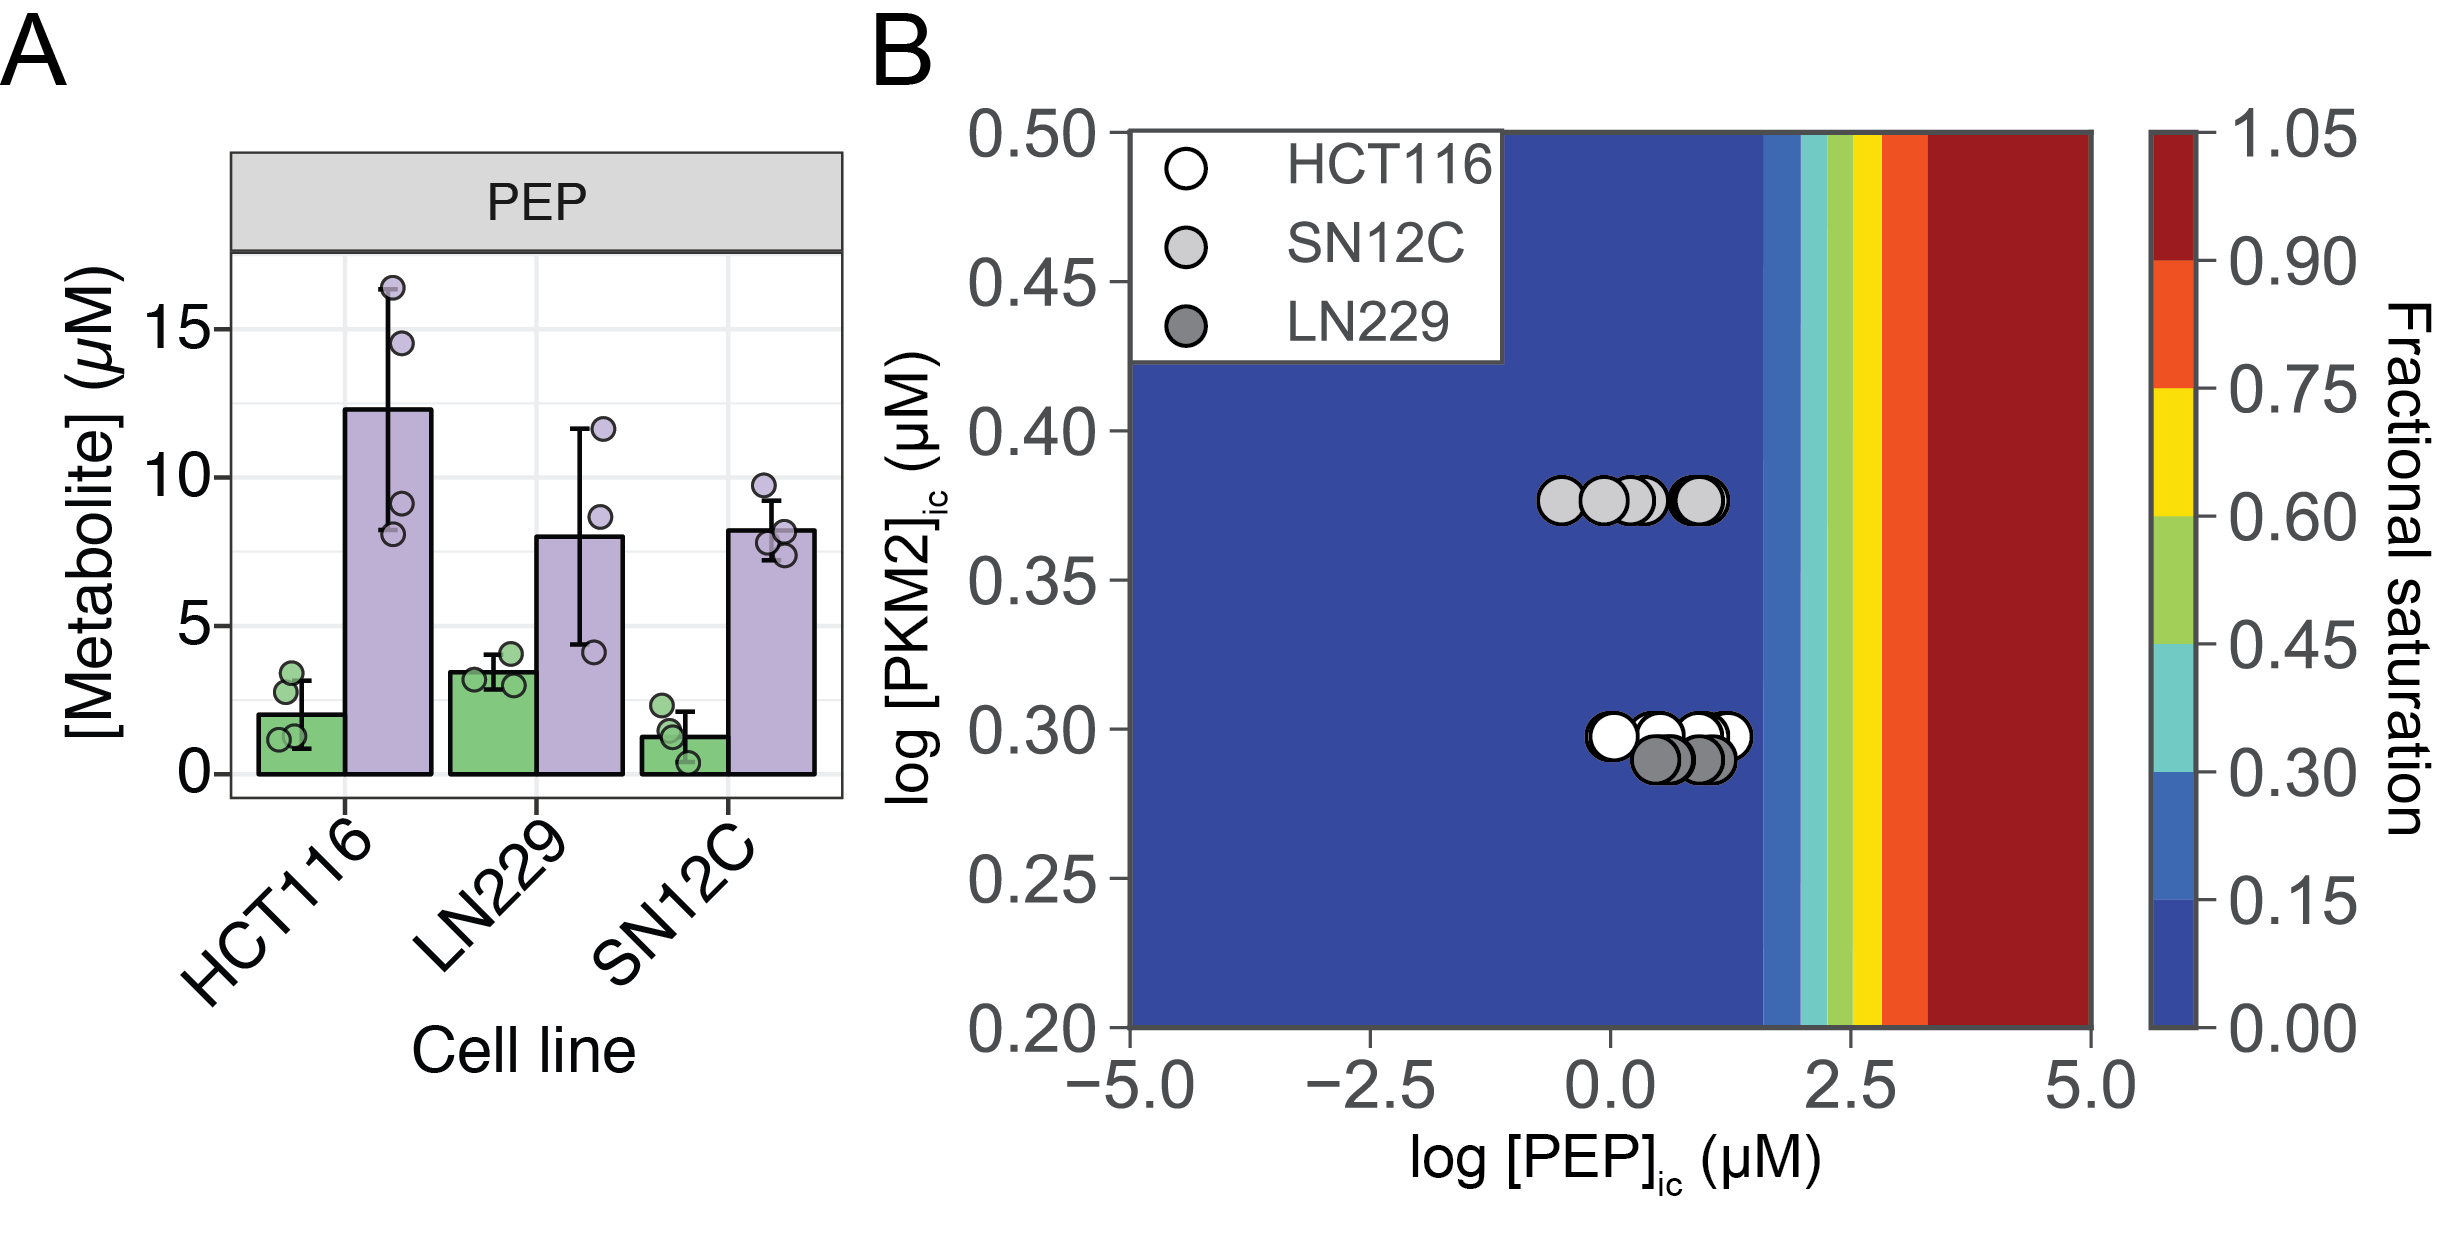
\includegraphics[scale=0.6]{ch4_fig12_pep_IC.png}
\caption[Intracellular concentrations of phosphoenolpyruvate are predicted to be constitutively limiting for PKM2 binding.] {\textbf{Intracellular concentrations of phosphoenolpyruvate are predicted to be constitutively limiting for PKM2 binding.} \textbf{(A)} Intracellular concentrations of phosphoenolpyruvate were determined in three cancer cell lines under 11 mM glucose-cultured (teal) and glucose-deprived (red) conditions. \textbf{(B)} A phase diagram of phosphoenolpyruvate binding to PKM2. A binding constant of 0.22 mM was used, as determined from PKM2 activity measurements under conditions of FBP binding.}
\label{fig:pep_conc}
\end{figure}
%
%
\clearpage

\subsection{High milli-molar phospho-peptide concentrations are required to reversibly displace FBP binding}
\label{subsec:pm2tide_kinetics}
In this chapter, it is shown that competition between Phe and Ser regulating the rate of $PKM2^{FBP}$ product turnover. The observed V-type effect of Phe and Ser is dependent on saturating FBP concentrations. We therefore reasoned that the combined regulatory effects of amino acids and FBP could be perturbed upon phosphopeptide-induced displacement of FBP binding. Nevertheless, exploring the stoichiometry of peptide binding to PKM2 in cells is complicated by the likelihood that multiple peptide binding motifs bind with varying affinities. Therefore, an accurate quantification of the fraction of PKM2 bound to phospho-peptides would require a comprehensive phospho-proteomics screen combined with a high-throughput peptide affinity effort, which was beyond the scope of this thesis. 
%
%
\\\\
%
%
Instead, to estimate the intracellular concentration of PKM2-binding phosphopeptide, required to reduce the binding affinity of FBP to levels which facilitate a non-constitutive phenotype, Equ. \ref{equ:saturation} was computed for a range of simulated phosphopeptide concentrations. It was assumed that all phosphopeptide molecules have the same binding affinity for PKM2, and that they all displace FBP with the same kinetics as measured in recombinant protein (see Section \ref{A phosphotyrosine peptide binds competitively with FBP to PKM2}). We found that phosphopeptide concentrations of approximately 40 mM were required to reduce the fractional saturation of FBP to 0.5 (\textbf{Fig. \ref{fig:peptide_sim}}).
%
%
\\\\
%
%
Together, these observations supported the hypothesis that, during steady-state cell proliferation under cell culture conditions, FBP is constitutively bound to PKM2. Under these conditions, amino acids can reversibly bind and thereby regulate the enzyme activity of PKM2 by modulating its maximal velocity, in the background of post-translational modifications that are likely to occur to PKM2 in cells.
%
%
%
%%% FIGURE
%
\begin{figure}[!ht]
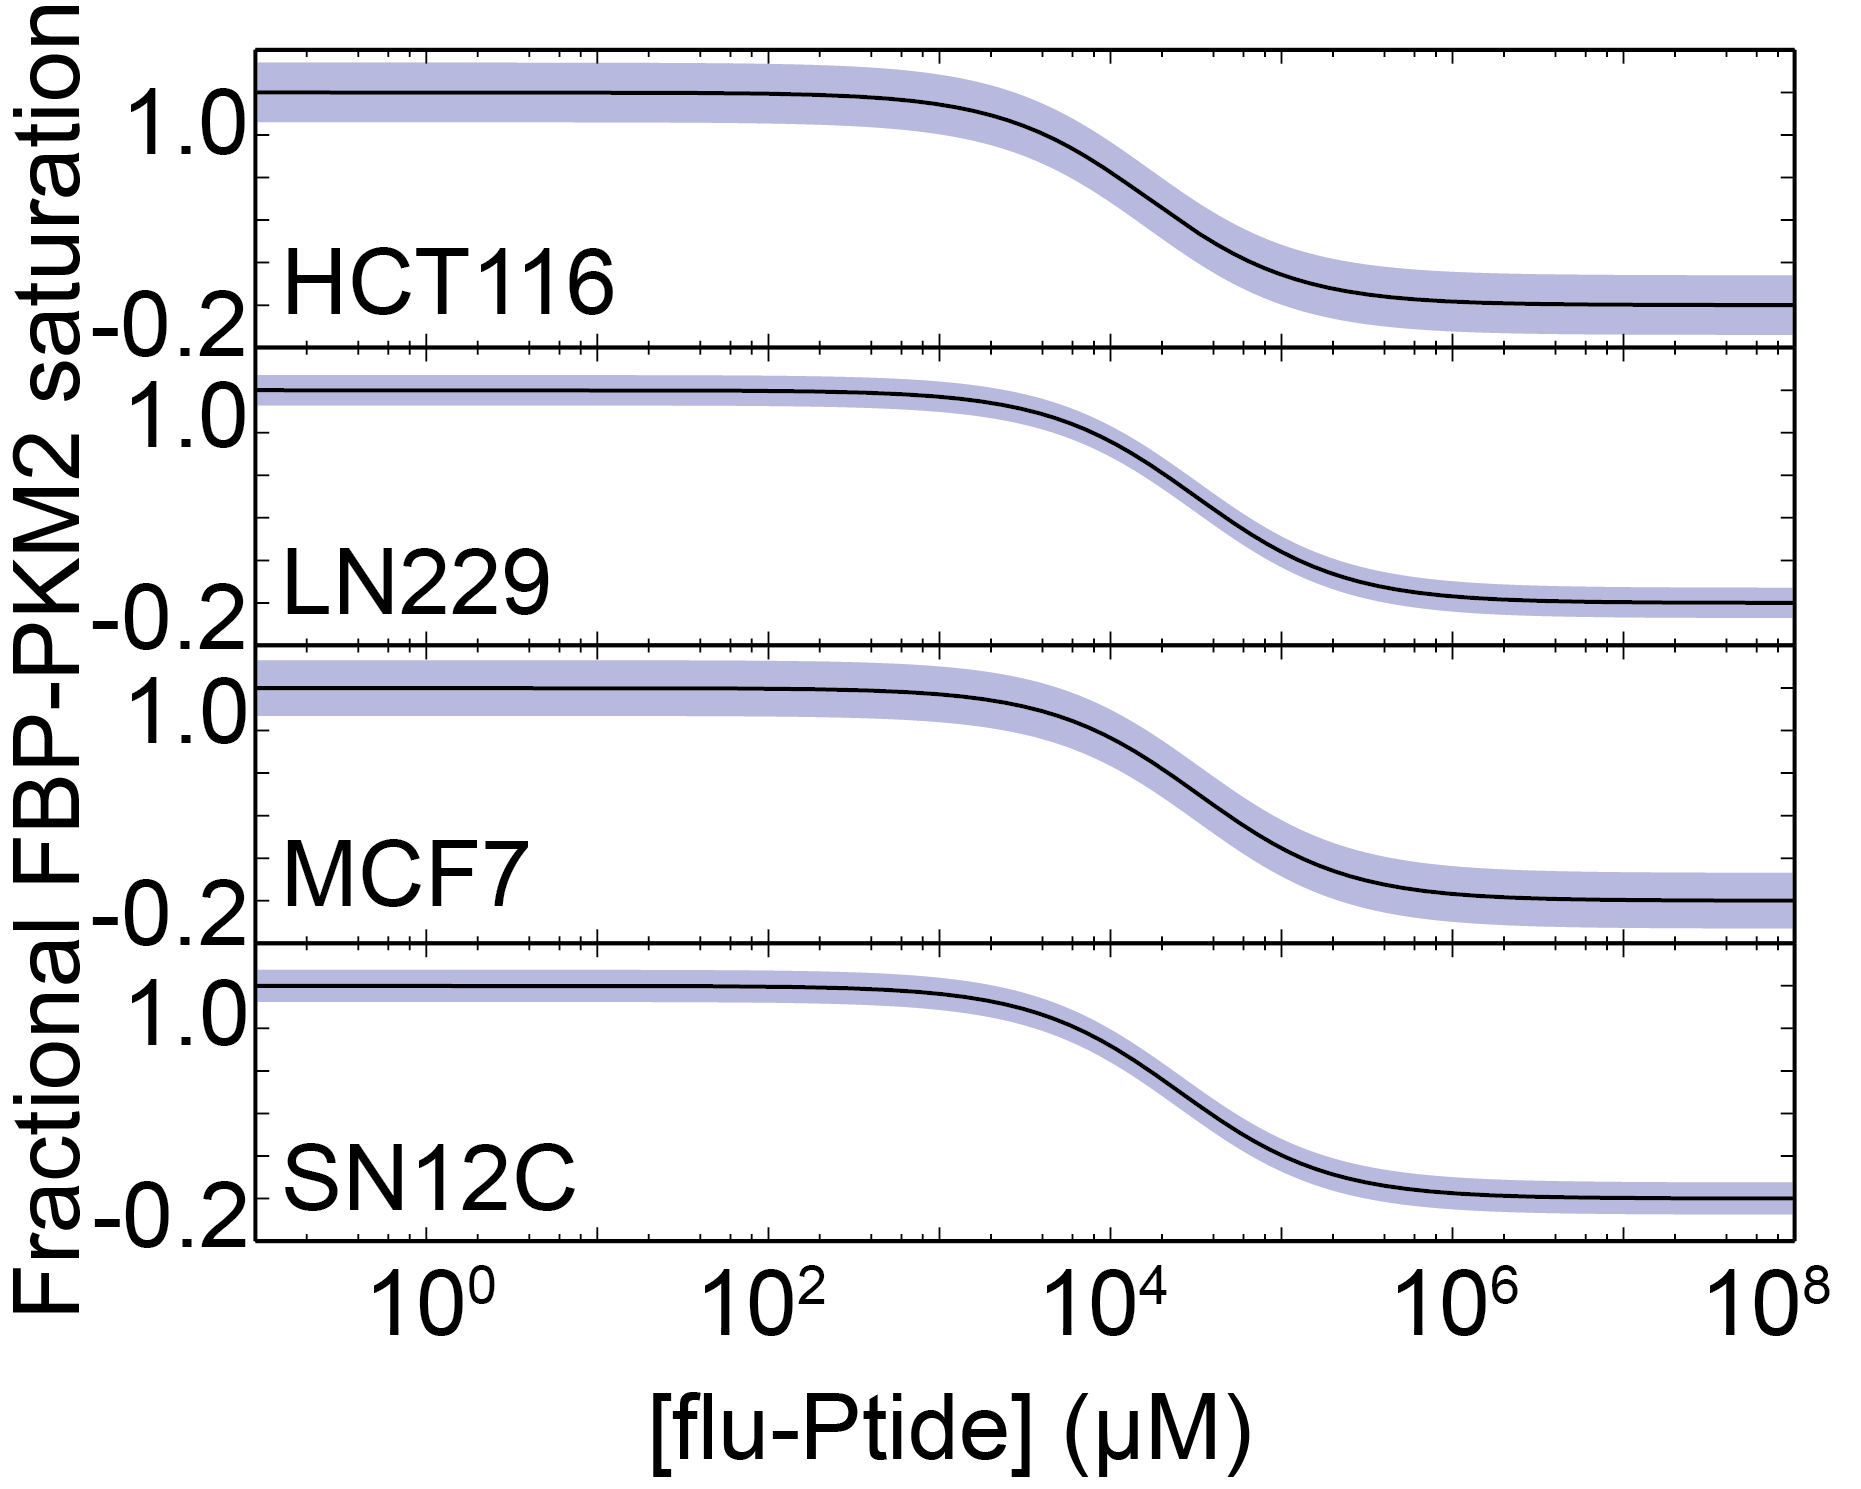
\includegraphics[scale=0.8]{ch4_fig13_peptide_simulation.png}
\caption[Milli-molar concentrations of phosphorylated peptide is required to out-compete FBP binding in cells.] {\textbf{Milli-molar concentrations of phosphorylated peptide is required to out-compete FBP binding in cells.} The fraction of PKM2 bound to FBP in HCT116, SN12C, MCF7 and LN229 cell lines was computed over a range of phospho-peptide concentrations.}
\label{fig:peptide_sim}
\end{figure}
%
%
\clearpage

\section{Conclusion}
Evidence, presented in this chapter, derived from measurements of PKM2 activity suggests that allosteric effectors can modulate the velocity and substrate affinity through a complex series of intra- and inter-protomeric couplings. Moreover, simultaneous regulation of PKM2 by FBP and amino acids is likely to occur over a large range of cell culture conditions. A major mechanism that has been suggested to result from allosteric effector binding is the regulation of the oligomeric state of PKM2. We therefore wanted to understand if, and to which extent, the findings of this chapter could be explained by ligand-induced oligomerisation of PKM2. We next turned to native mass spectrometry to investigate the potential of allosteric regulators to effect changes in the oligomeric state of PKM2.



















 
